\documentclass[a4paper, 12pt]{article}
\usepackage[utf8x]{inputenc}
\usepackage{cmap}
\usepackage[english, russian]{babel}
\usepackage{indentfirst}
\usepackage[left=20mm, top=20mm, right=20mm, bottom=20mm]{geometry}
\usepackage{tikz}
\usepackage{float}
\usepackage{amsmath, amsfonts, amssymb}
\usepackage{graphicx}
\usepackage{fancybox, fancyhdr}
\usepackage{hyperref}
\usepackage{listings}
\usepackage{caption}
\usepackage{subcaption}
\usepackage{xcolor}
\pagestyle{fancy}
\fancyhf{}
\fancyhead[L]{Лабораторная работа №3}
\fancyhead[R]{Частотные методы}
\fancyfoot[C]{\thepage}
\graphicspath{{images/}}
\usetikzlibrary{patterns}
\definecolor{LightGray}{gray}{0.95}
\lstdefinestyle{pycode}{
    language=Python,
    basicstyle=\footnotesize\ttfamily,
    numbers=left,
    numberstyle=\tiny\color{gray},
    stepnumber=1,
    numbersep=5pt,
    backgroundcolor=\color{LightGray},
    showspaces=false,
    showstringspaces=false,
    showtabs=false,
    tabsize=4,
    captionpos=b,
    breaklines=true,
    breakatwhitespace=false,
    frame=none,
    rulecolor=\color{black},
    linewidth=\linewidth,
    keywordstyle=\color{red}\bfseries,
    commentstyle=\color{green!40!black},
    stringstyle=\color{blue},
    escapeinside={\%*}{*)},
    xleftmargin=0pt,
    framexleftmargin=0pt,
    framexrightmargin=0pt
}
\lstset{style=pycode}
\hypersetup{
    colorlinks=true,
    linkcolor=blue,
    filecolor=magenta,      
    urlcolor=cyan,
    pdftitle={contents setup},
    pdfpagemode=FullScreen,
}
\setlength{\parskip}{1.5mm}
\setlength{\headheight}{15pt}
\setlength{\footskip}{15pt}
\allowdisplaybreaks
\DeclareMathOperator{\sinc}{sinc}
\newcommand{\frc}[2]{\raisebox{2pt}{$#1$}\big/\raisebox{-3pt}{$#2$}}

\begin{document}
    \begin{titlepage}

        \begin{center}
        
\includegraphics[width=0.3\textwidth]{itmo.png} % requires itmo.png in /images folder
        \vfill
        
        Федеральное государственное автономное образовательное учреждение высшего образования
        «Национальный Исследовательский Университет ИТМО»\\
        
        \vfill
        {\large\bf ЛАБОРАТОРНАЯ РАБОТА №3}\\
        {\large\bf ПРЕДМЕТ «ЧАСТОТНЫЕ МЕТОДЫ»}\\
        {\large\bf ТЕМА «ЖЕСТКАЯ ФИЛЬТРАЦИЯ»}
        \vfill

        \begin{flushright}
            \begin{minipage}{.45\textwidth}
            {
                \hbox{Лектор: Перегудин А. А.}
                \hbox{Практик: Пашенко А. В.}
                \hbox{Студент: Румянцев А. А.}
                \hbox{Поток: ЧАСТ.МЕТ. 1.3}
                \hbox{}
                \hbox{Факультет: СУиР}
                \hbox{Группа: R3241}
            }
            \end{minipage}
        \end{flushright}
        
        \vfill
                
        Санкт-Петербург\\
        2024
        \end{center}
    \end{titlepage}
    
    \tableofcontents

    \newpage
% \end{document}
    \section{Задание 1. Жесткие фильтры}
    В этом задании выполним жесткую фильтрацию сигнала. Для этого будем находить Фурье-образ сигнала, обнулять его значения
    на некоторых диапазонах частот, затем восстанавливать сигнал с помощью обратного преобразования.


    Зададим такие числа $a,\,t_1,\,t_2$, что $t_1<t_2$, и рассмотрим функцию $g$ такую, что
    $g(t)=a$ при $t\in[t_1,t_2]$ и $g(t)=0$ при других $t$. $$\sqsupset a=2,\ \ t_1=-1.5,\ \ t_2=2.5,\ \ g(t)=
    \begin{cases}
        2, & t\in[t_1,t_2]\\
        0, & \text{ otherwise}
    \end{cases}
    $$


    Выберем интервал времени $T=10$ и шаг дискретизации $dt=0.01$. Зададим в python массив времени $t$ от $-0.5\cdot T$ до $0.5\cdot T+dt$
    с шагом $dt$ и включим последнюю точку. Найдем список значений $g(t)$ и зададим зашумленную версию сигнала как
    $$
    u=g(t)+b\cdot(\text{random}(\text{len}(t))-0.5) + c\cdot \sin(d\cdot t);
    $$


    В заданном сигнале параметр $a$ функции $g(t)$ отвечает за высоту, на которую поднимется часть сигнала от нуля на промежутке $[t_1,t_2]$.
    Оставшиеся параметры вносят различные виды шума в сигнал.


    \subsection{Убираем высокие частоты. Фильтр нижних частот}
    Положим параметр $c=0$. Возьмем некоторый диапазон частот $[-\nu_0, \nu_0]$, на котором оставим Фурье-образ
    сигнала $u$ неизменным, а на остальных частотах обнулим его значения. То есть применим фильтр \textit{нижних} частот -- он пропускает
    все частоты ниже частоты среза. Построим сравнительные графики исходного и фильтрованного сигналов, а также модулей
    их Фурье-образов. Исследуем влияние частоты среза $\nu_0$ и значения параметра $b$ на эффективность фильтрации.
    
    
    Далее будут приведены рисунки полученных графиков. На каждом графике подписаны выбранные значения $b,\,c,\,d,\,\nu_0$.
    Синим цветом обозначается оригинальный сигнал, красным фильтрованный.


    \begin{figure}[H]
        \centering
        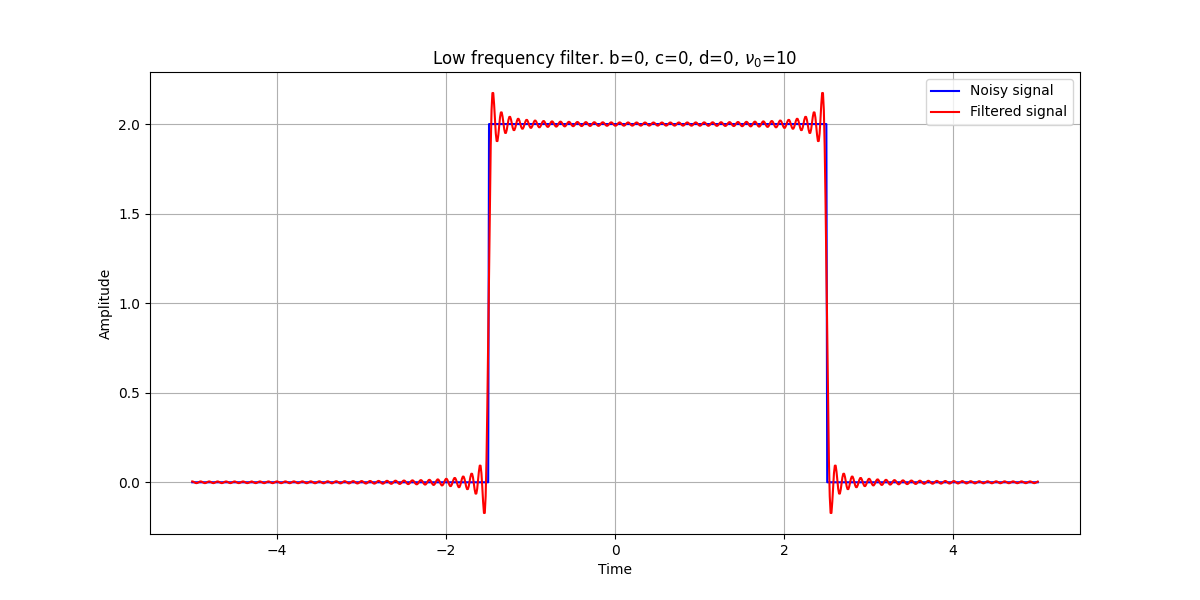
\includegraphics[scale=0.48]{1_nohigh.png}
        \captionsetup{skip=0pt}
        \caption{График исходного и фильтрованного сигналов (1)}
        \label{fig:fig1}
    \end{figure}
    \begin{figure}[H]
        \centering
        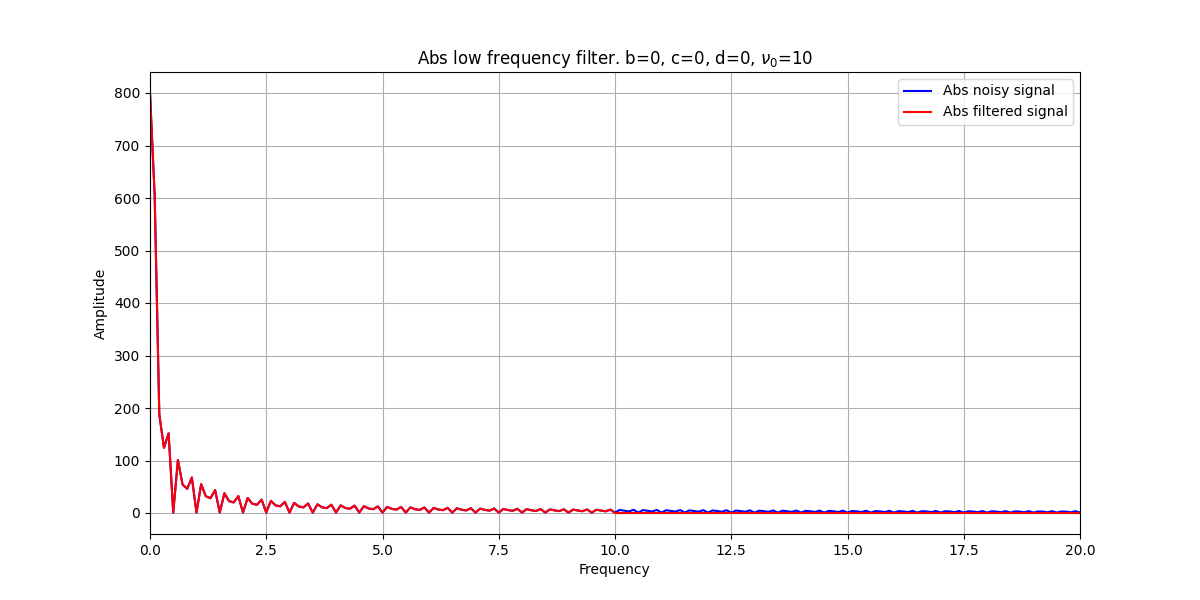
\includegraphics[scale=0.48]{1_abs_nohigh.png}
        \captionsetup{skip=0pt}
        \caption{График модуля Фурье-образа исходного и фильтрованного сигналов (1)}
        \label{fig:fig2}
    \end{figure}
    \begin{figure}[H]
        \centering
        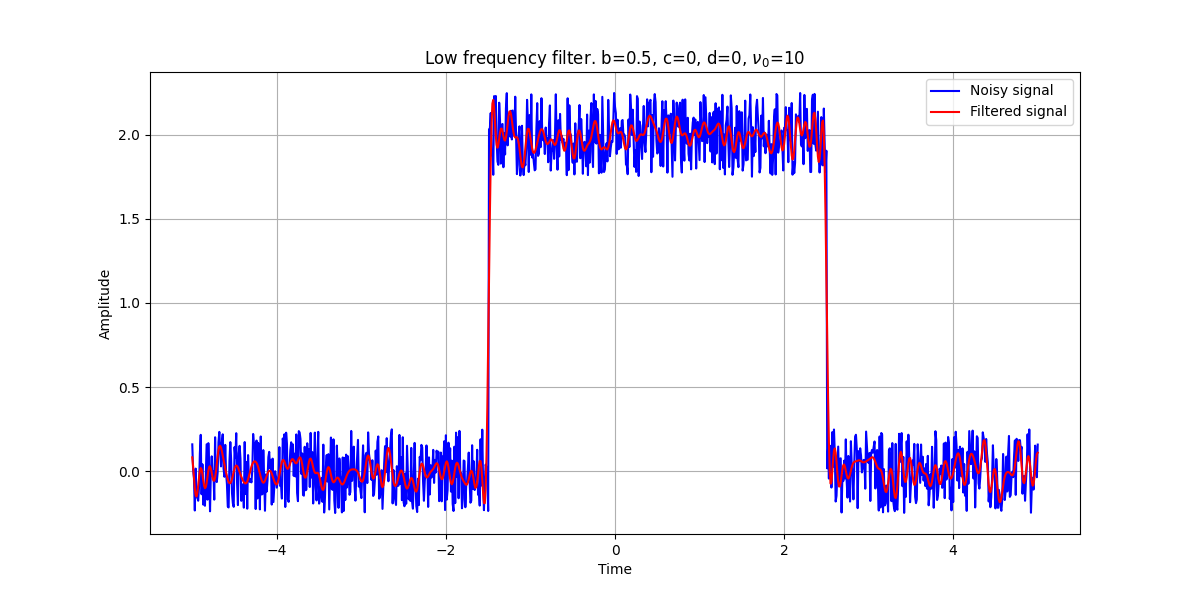
\includegraphics[scale=0.48]{2_nohigh.png}
        \captionsetup{skip=0pt}
        \caption{График исходного и фильтрованного сигналов (2)}
        \label{fig:fig3}
    \end{figure}
    \begin{figure}[H]
        \centering
        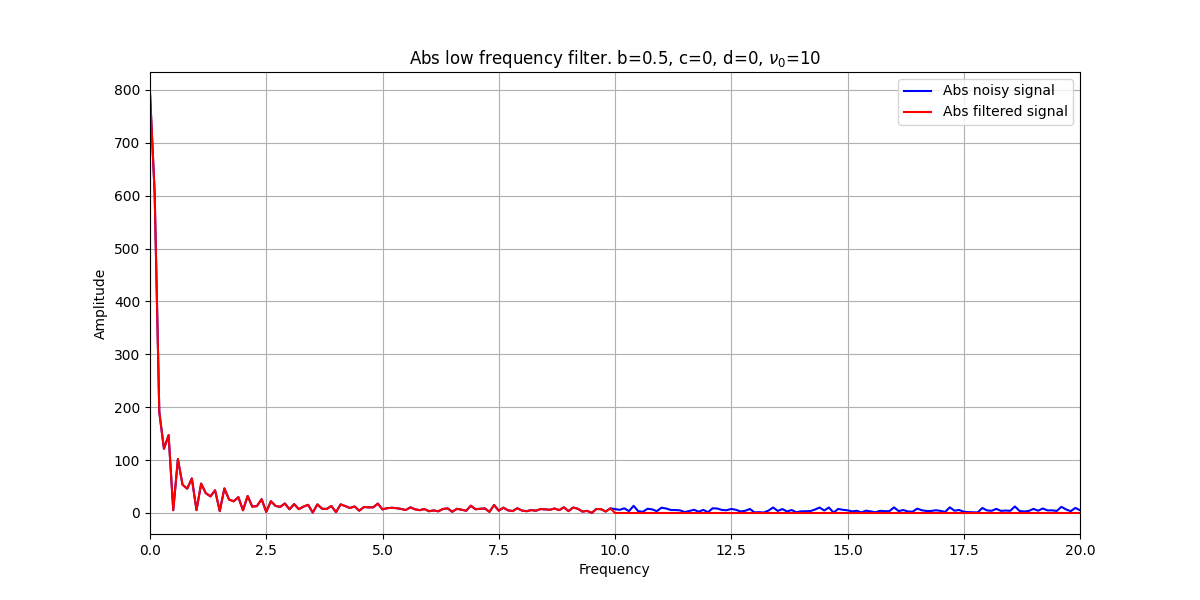
\includegraphics[scale=0.48]{2_abs_nohigh.png}
        \captionsetup{skip=0pt}
        \caption{График модуля Фурье-образа исходного и фильтрованного сигналов (2)}
        \label{fig:fig4}
    \end{figure}
    \begin{figure}[H]
        \centering
        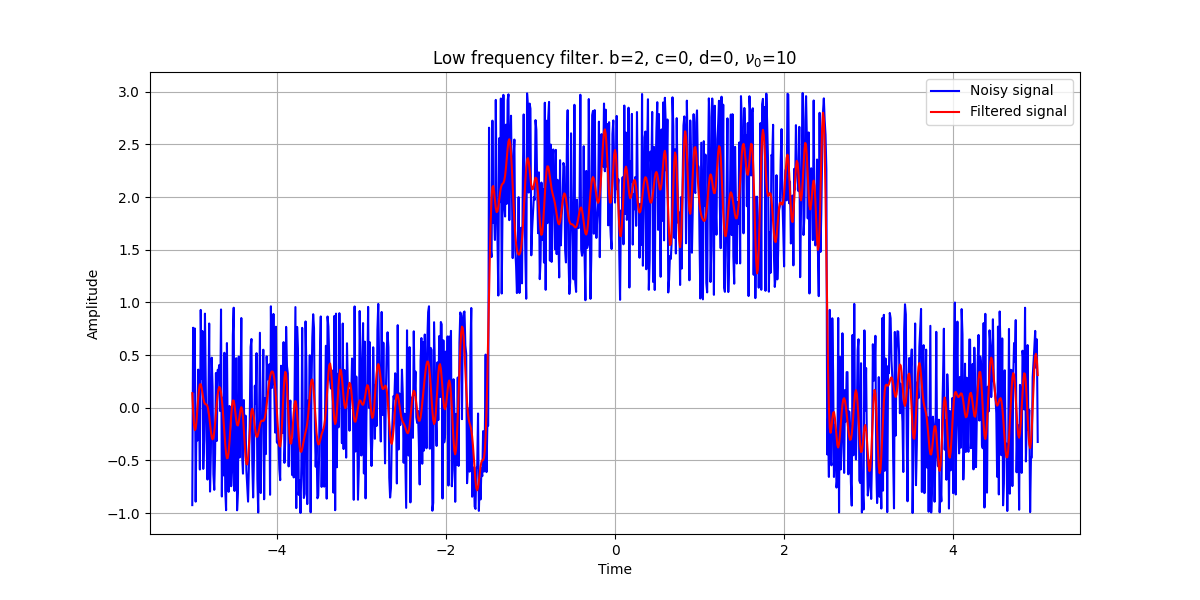
\includegraphics[scale=0.48]{3_nohigh.png}
        \captionsetup{skip=0pt}
        \caption{График исходного и фильтрованного сигналов (3)}
        \label{fig:fig5}
    \end{figure}
    \begin{figure}[H]
        \centering
        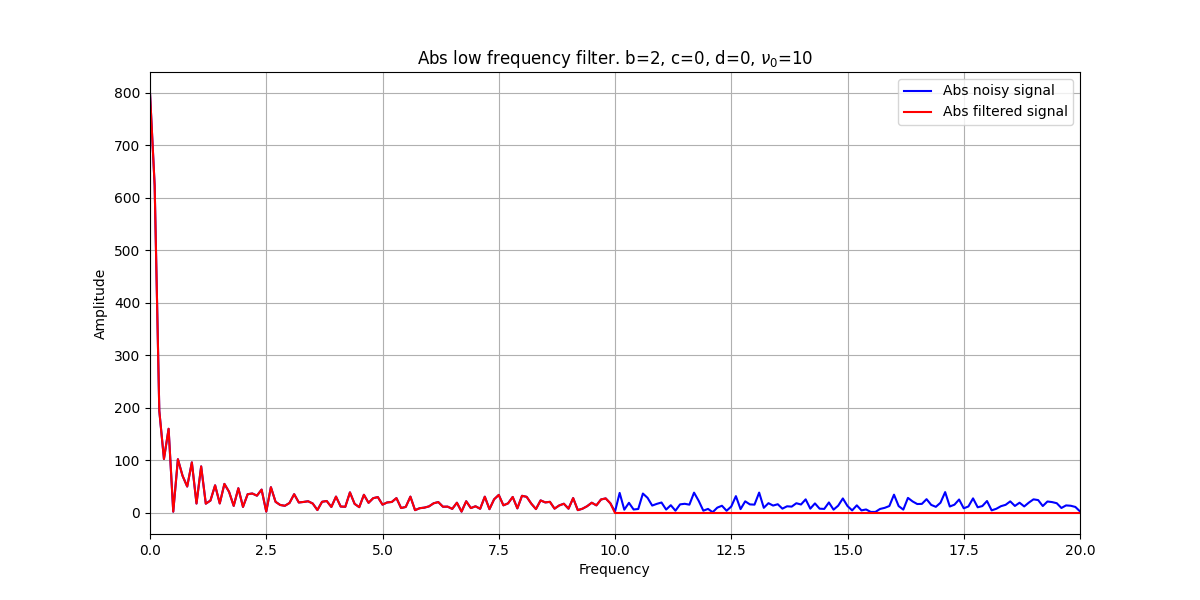
\includegraphics[scale=0.48]{3_abs_nohigh.png}
        \captionsetup{skip=0pt}
        \caption{График модуля Фурье-образа исходного и фильтрованного сигналов (3)}
        \label{fig:fig6}
    \end{figure}
    \begin{figure}[H]
        \centering
        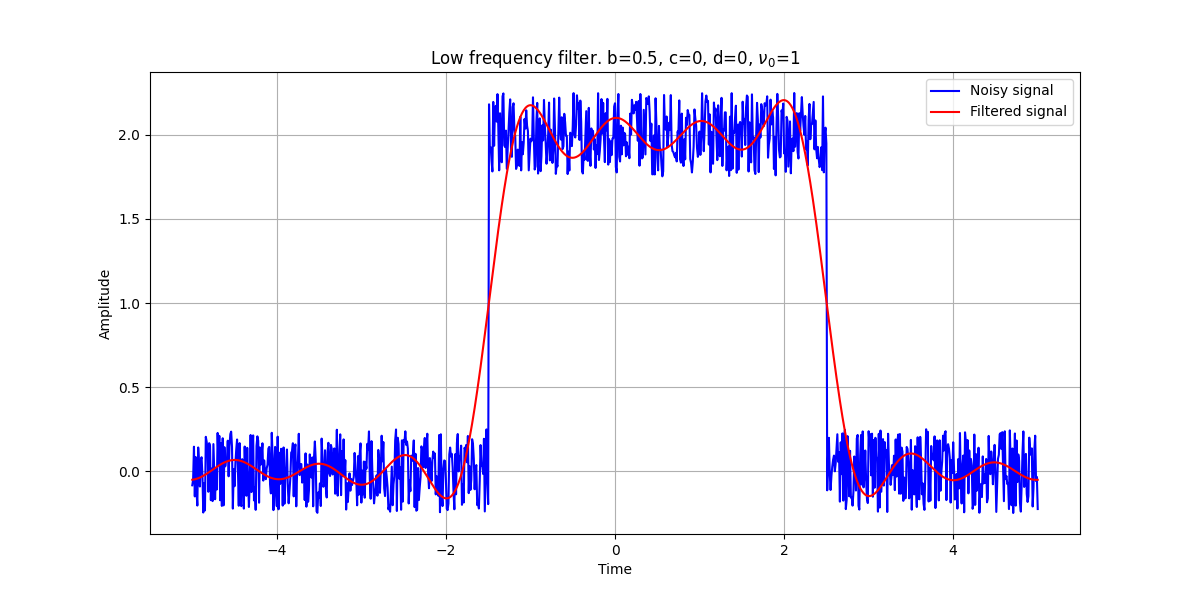
\includegraphics[scale=0.48]{4_nohigh.png}
        \captionsetup{skip=0pt}
        \caption{График исходного и фильтрованного сигналов (4)}
        \label{fig:fig7}
    \end{figure}
    \begin{figure}[H]
        \centering
        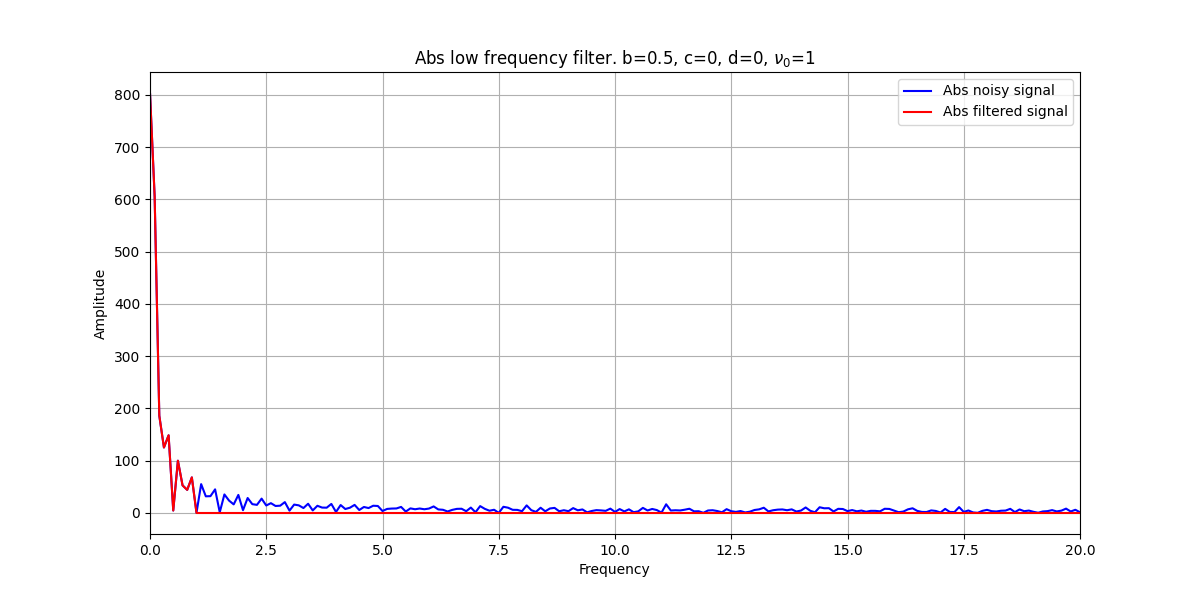
\includegraphics[scale=0.48]{4_abs_nohigh.png}
        \captionsetup{skip=0pt}
        \caption{График модуля Фурье-образа исходного и фильтрованного сигналов (4)}
        \label{fig:fig8}
    \end{figure}
    \begin{figure}[H]
        \centering
        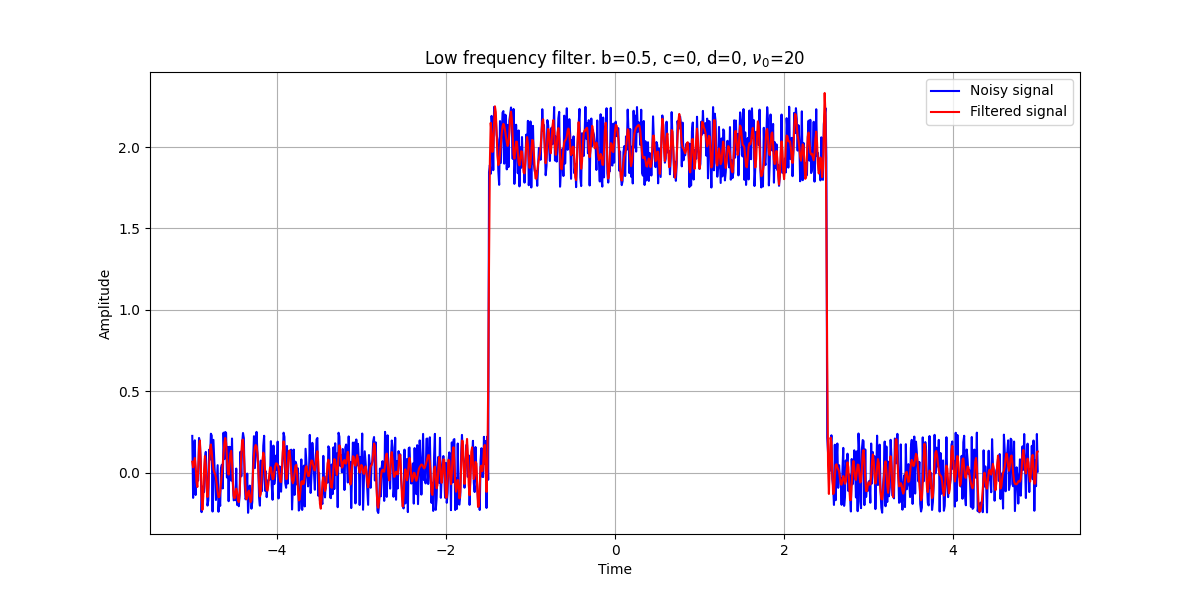
\includegraphics[scale=0.48]{5_nohigh.png}
        \captionsetup{skip=0pt}
        \caption{График исходного и фильтрованного сигналов (5)}
        \label{fig:fig9}
    \end{figure}
    \begin{figure}[H]
        \centering
        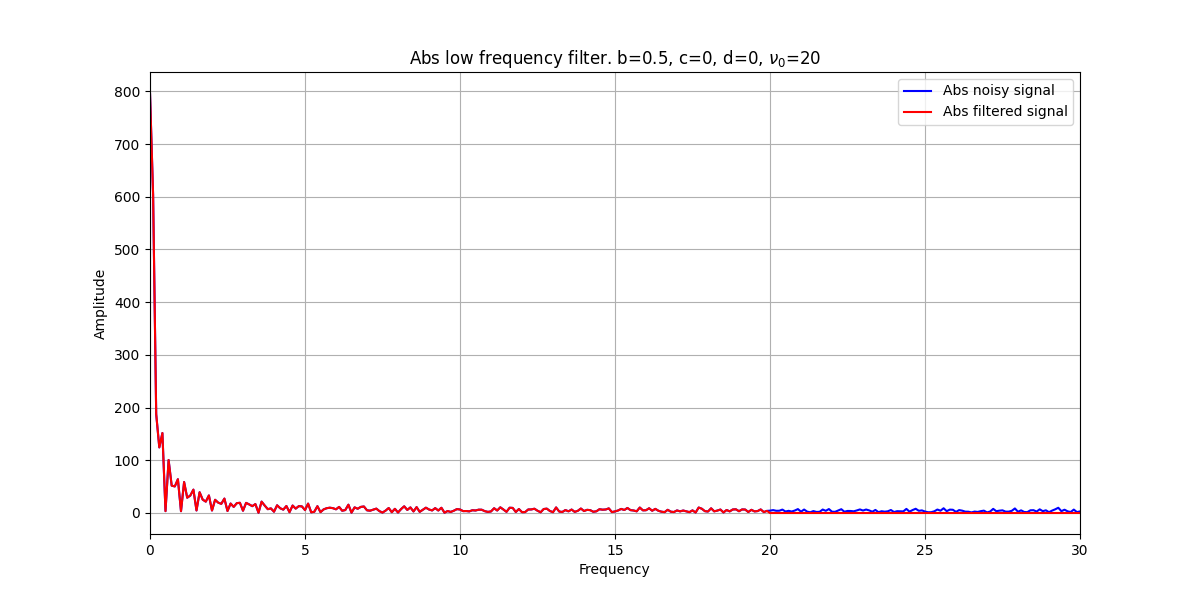
\includegraphics[scale=0.48]{5_abs_nohigh.png}
        \captionsetup{skip=0pt}
        \caption{График модуля Фурье-образа исходного и фильтрованного сигналов (5)}
        \label{fig:fig10}
    \end{figure}


    Исходя из графиков можно сделать вывод, что значение параметра $b$ отвечает за белый шум.
    Чем больше значение $b$, тем больше белого шума (сравн. рис. \ref{fig:fig1}, \ref{fig:fig3}, \ref{fig:fig5}) --
    сложнее фильтровать сигнал, так как увеличивается его концентрация в значащих частотах. В данном случае
    основная информация о сигнале находится на нижних частотах вблизи нуля -- это мы видим на графиках Фурье-образов.
    При $b=0$ сигнал становится прямоугольной функцией. Фильтрация такого сигнала выглядит как ее аппроксимация (см. рис. \ref{fig:fig1}).
    При большом значении $b$ исходный сигнал восстановить не получится.


    Эффективность фильтрации зависит от выбора частоты среза $\nu_0$. Зададим маленький диапазон --
    вырежем б\'{о}льшую часть шума и часть нужного сигнала (см. рис. \ref{fig:fig8}). Большой диапазон оставит и сигнал и некоторую
    часть шума, которую можно было вырезать (см. рис. \ref{fig:fig10}). Значение, сохраняющее наибольшее количество
    значащих частот, будет являться оптимальным и даст наилучшую фильтрацию.


    \subsection{Убираем специфические частоты. Режекторный фильтр}
    Возьмем ненулевые параметры $b,\,c,\,d$. Попробуем
    обнулять некоторые диапазоны частот, а также
    совместим различные варианты фильтрации, чтобы по возможности убрать влияние обеих компонент помехи.
    Исследуем влияние частот среза и значений параметров $b,\,c,\,d$ на вид помехи и эффективность
    фильтрации. Отдельно рассмотрим случай для $b=0$.


    Синусоидальный шум отображается на графике Фурье-образа как высокий пик помимо исходного, который мы наблюдали ранее в диапазоне низких частот
    и который содержит наибольшее количество информации об исходном сигнале. Чтобы увидеть этот дополнительный высокий пик, необходимо взять немаленькое значение параметра $d$.
    Обнулим частоты в его диапазоне и посмотрим результат. Должен
    получиться сигнал, похожий на прямоугольную функцию. Также совместим фильтрацию специфических частот с низкими, то есть уберем высокие, которые
    несут наименьшее количество информации об исходном сигнале, но вносят значительный шум.


    Далее будут приведены рисунки полученных графиков. На каждом графике подписаны выбранные значения $b,\,c,\,d,\,\nu_0$. 
    Синим цветом обозначается оригинальный сигнал, красным фильтрованный. 


    \begin{figure}[H]
        \centering
        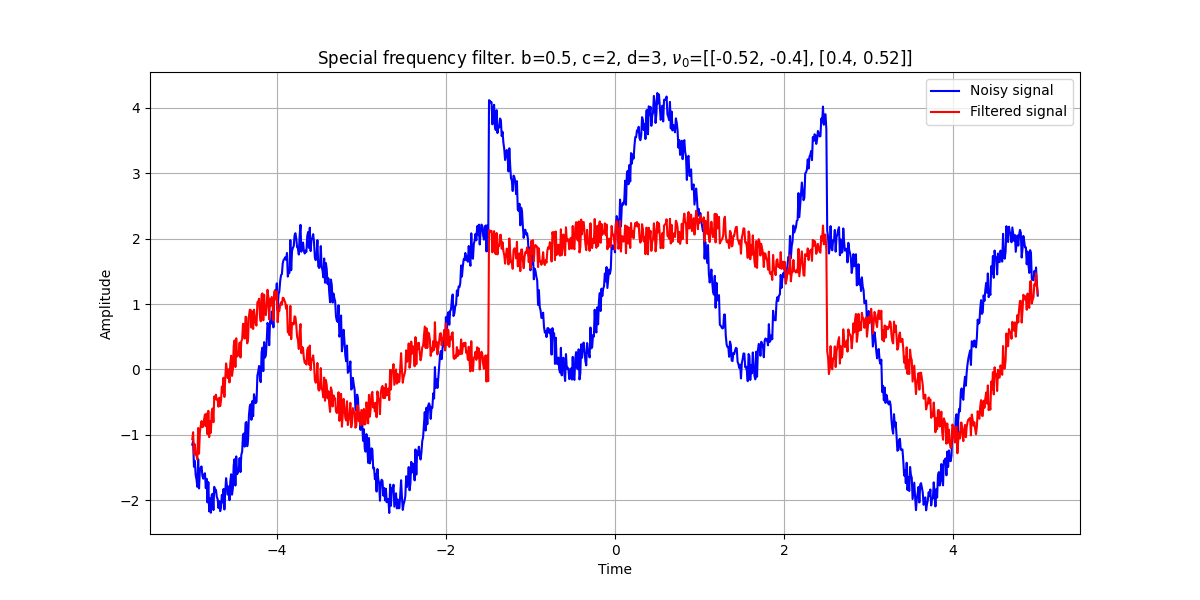
\includegraphics[scale=0.48]{1_nospec.png}
        \captionsetup{skip=0pt}
        \caption{График исходного и фильтрованного сигналов (1.1)}
        \label{fig:fig71}
    \end{figure}
    \begin{figure}[H]
        \centering
        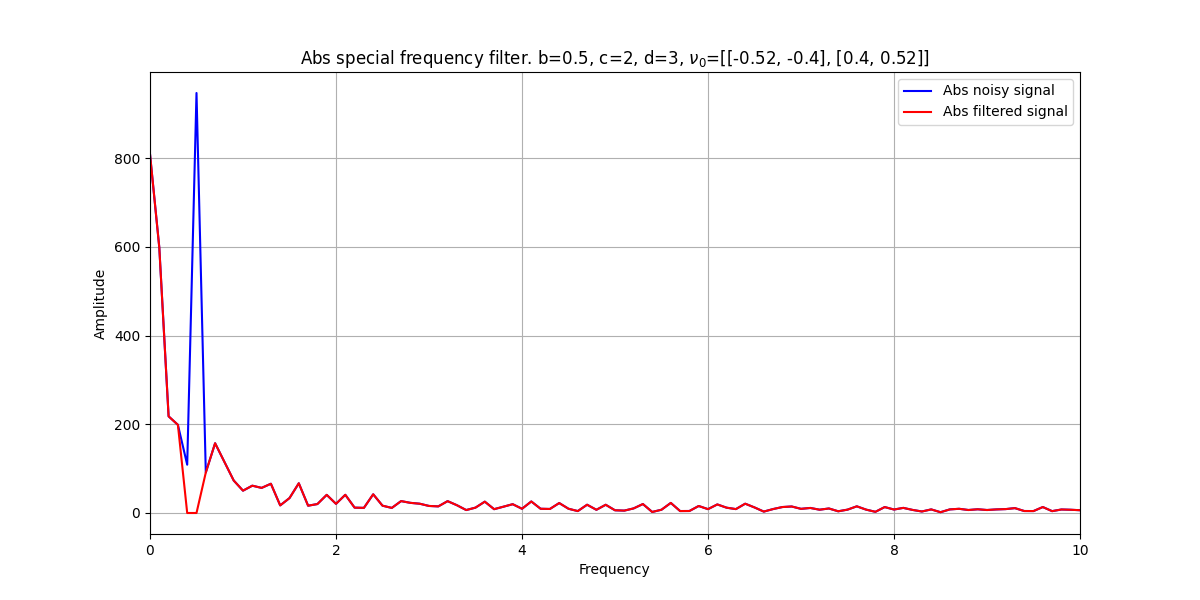
\includegraphics[scale=0.48]{1_abs_nospec.png}
        \captionsetup{skip=0pt}
        \caption{График модуля Фурье-образа исходного и фильтрованного сигналов (1.1)}
        \label{fig:fig72}
    \end{figure}
    \begin{figure}[H]
        \centering
        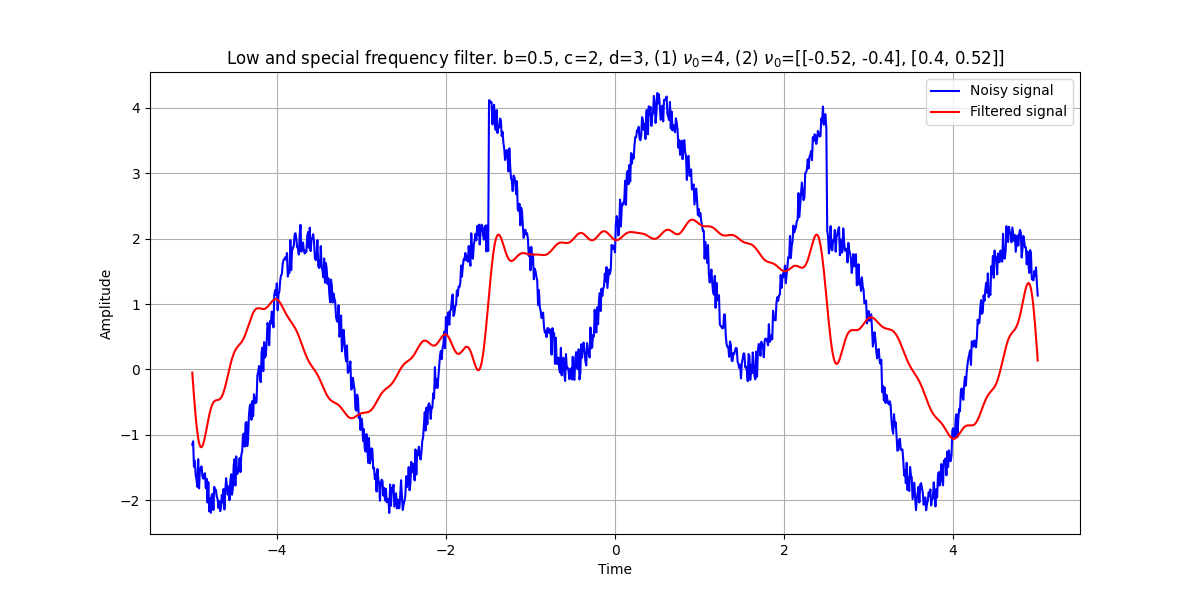
\includegraphics[scale=0.48]{1_nospec_nohigh.png}
        \captionsetup{skip=0pt}
        \caption{График исходного и фильтрованного сигналов (1.2)}
        \label{fig:fig77}
    \end{figure}
    \begin{figure}[H]
        \centering
        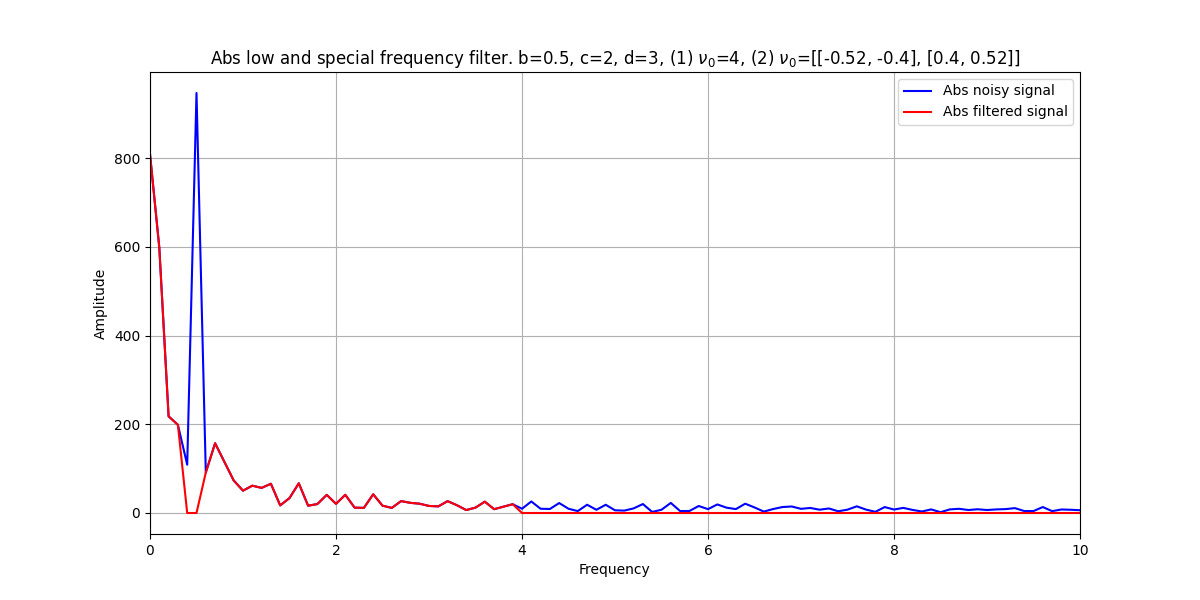
\includegraphics[scale=0.48]{1_abs_nospec_nohigh.png}
        \captionsetup{skip=0pt}
        \caption{График модуля Фурье-образа исходного и фильтрованного сигналов (1.2)}
        \label{fig:fig78}
    \end{figure}
    \begin{figure}[H]
        \centering
        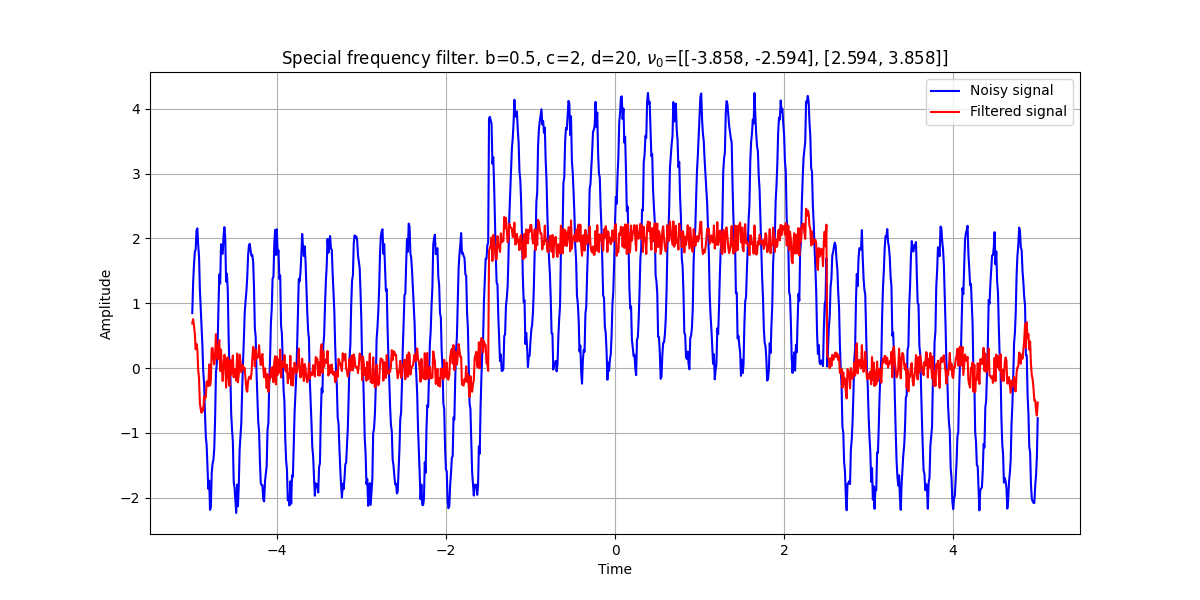
\includegraphics[scale=0.48]{2_nospec.png}
        \captionsetup{skip=0pt}
        \caption{График исходного и фильтрованного сигналов (2.1)}
        \label{fig:fig712}
    \end{figure}
    \begin{figure}[H]
        \centering
        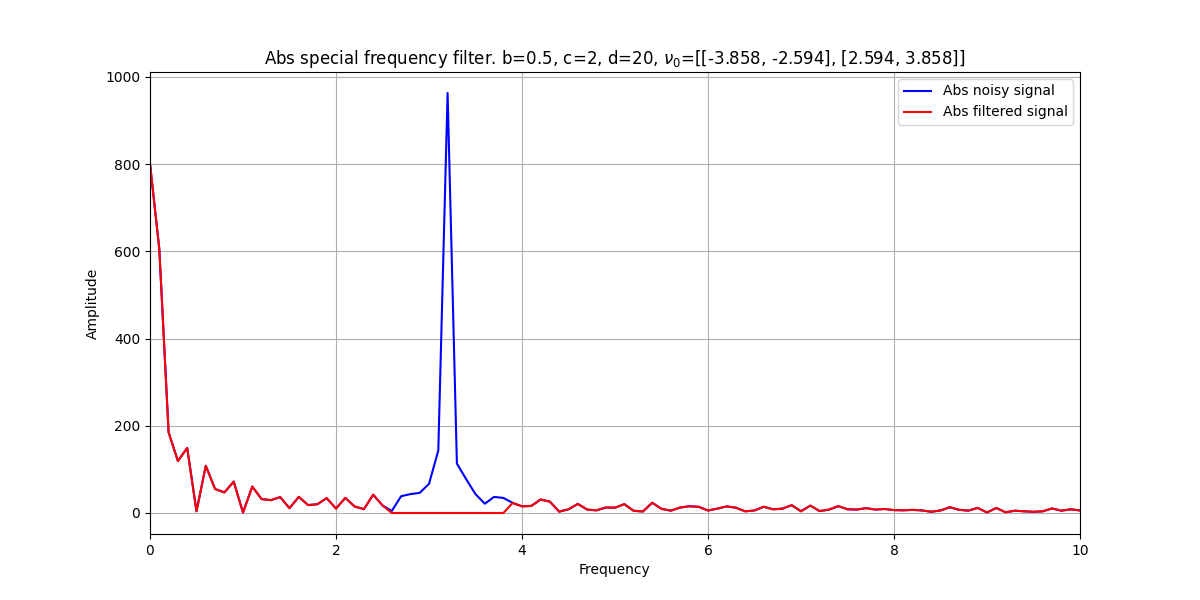
\includegraphics[scale=0.48]{2_abs_nospec.png}
        \captionsetup{skip=0pt}
        \caption{График модуля Фурье-образа исходного и фильтрованного сигналов (2.1)}
        \label{fig:fig722}
    \end{figure}
    \begin{figure}[H]
        \centering
        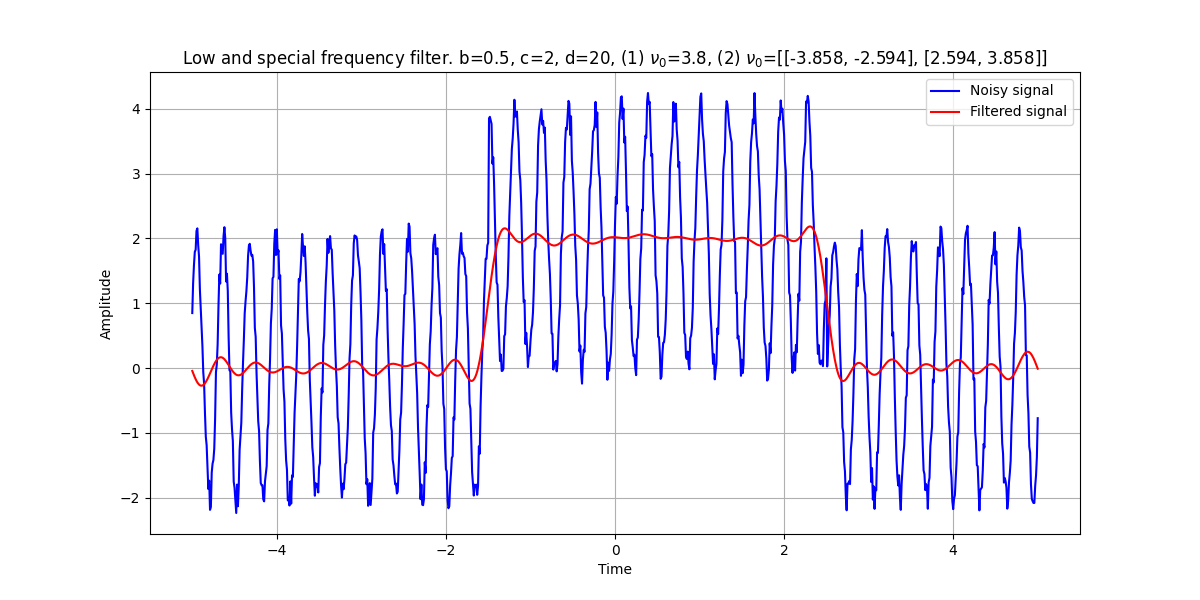
\includegraphics[scale=0.48]{2_nospec_nohigh.png}
        \captionsetup{skip=0pt}
        \caption{График исходного и фильтрованного сигналов (2.2)}
        \label{fig:fig772}
    \end{figure}
    \begin{figure}[H]
        \centering
        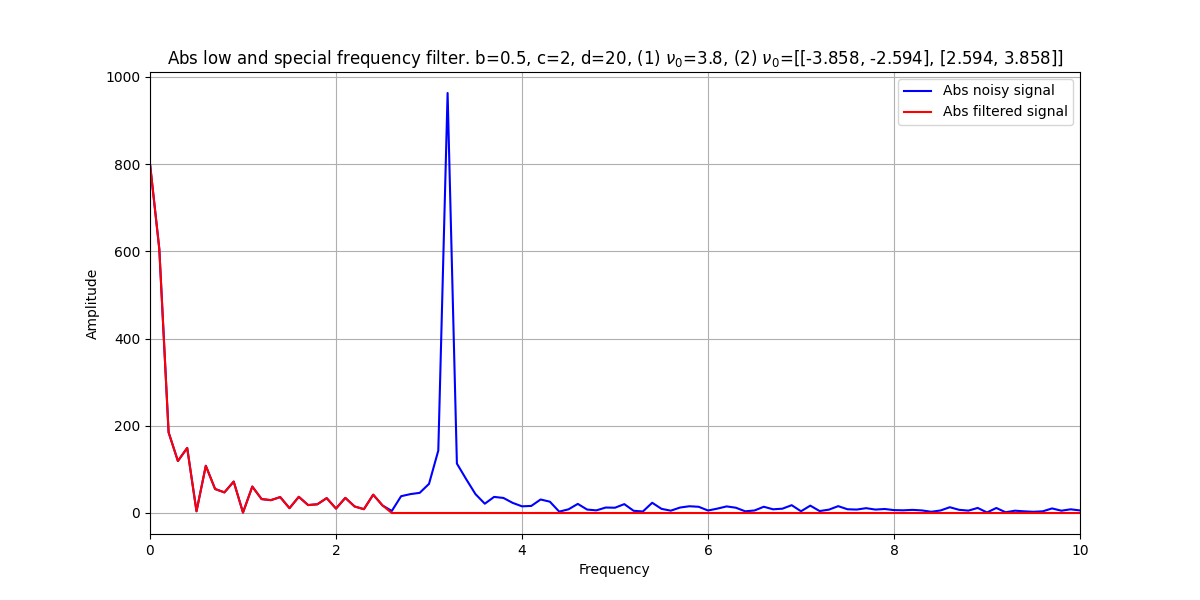
\includegraphics[scale=0.48]{2_abs_nospec_nohigh.png}
        \captionsetup{skip=0pt}
        \caption{График модуля Фурье-образа исходного и фильтрованного сигналов (2.2)}
        \label{fig:fig782}
    \end{figure}
    \begin{figure}[H]
        \centering
        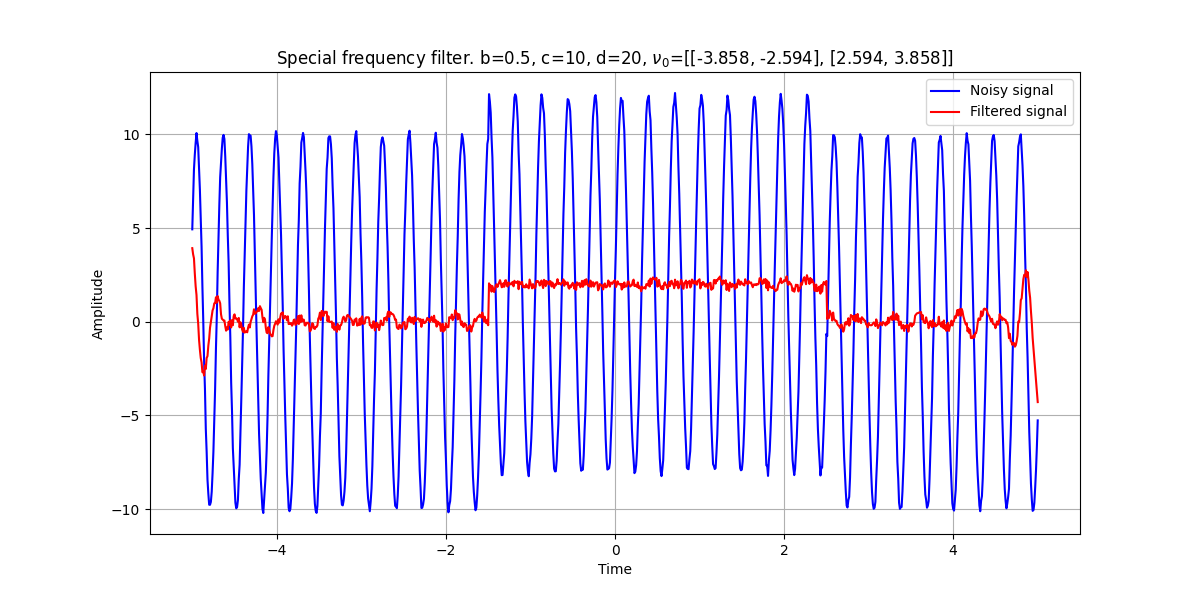
\includegraphics[scale=0.48]{3_nospec.png}
        \captionsetup{skip=0pt}
        \caption{График исходного и фильтрованного сигналов (3.1)}
        \label{fig:fig7123}
    \end{figure}
    \begin{figure}[H]
        \centering
        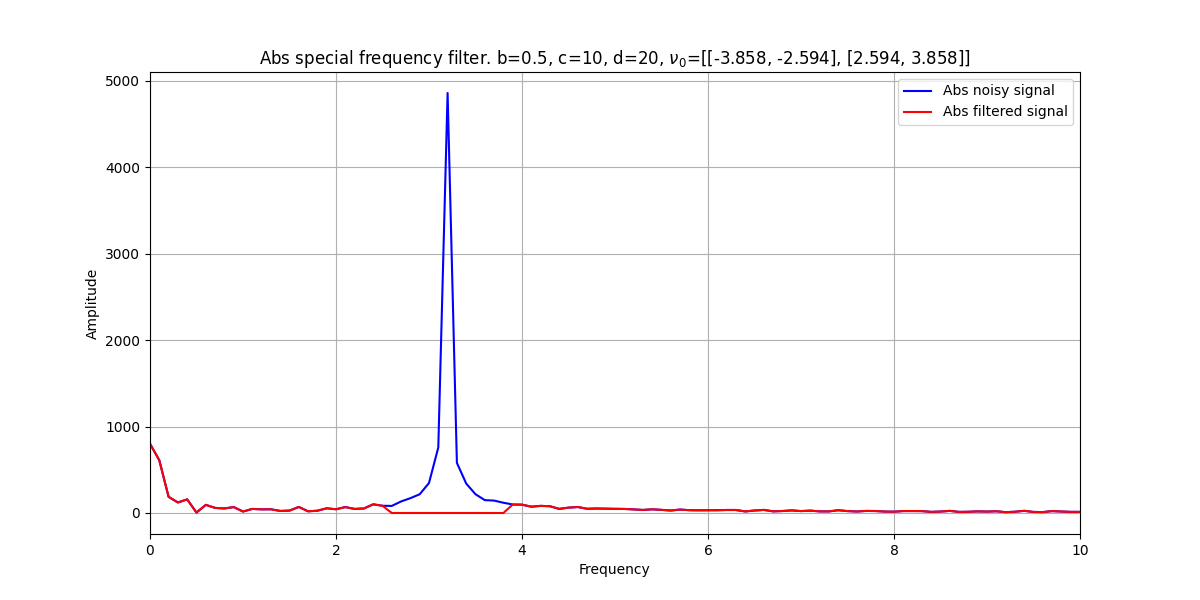
\includegraphics[scale=0.48]{3_abs_nospec.png}
        \captionsetup{skip=0pt}
        \caption{График модуля Фурье-образа исходного и фильтрованного сигналов (3.1)}
        \label{fig:fig7223}
    \end{figure}
    \begin{figure}[H]
        \centering
        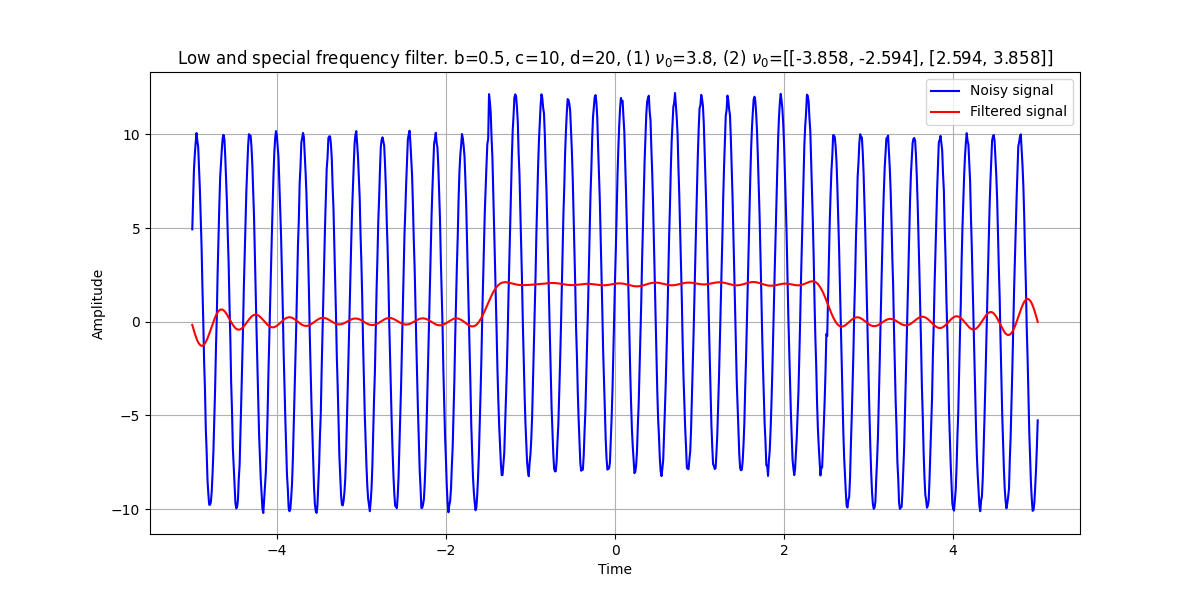
\includegraphics[scale=0.48]{3_nospec_nohigh.png}
        \captionsetup{skip=0pt}
        \caption{График исходного и фильтрованного сигналов (3.2)}
        \label{fig:fig7723}
    \end{figure}
    \begin{figure}[H]
        \centering
        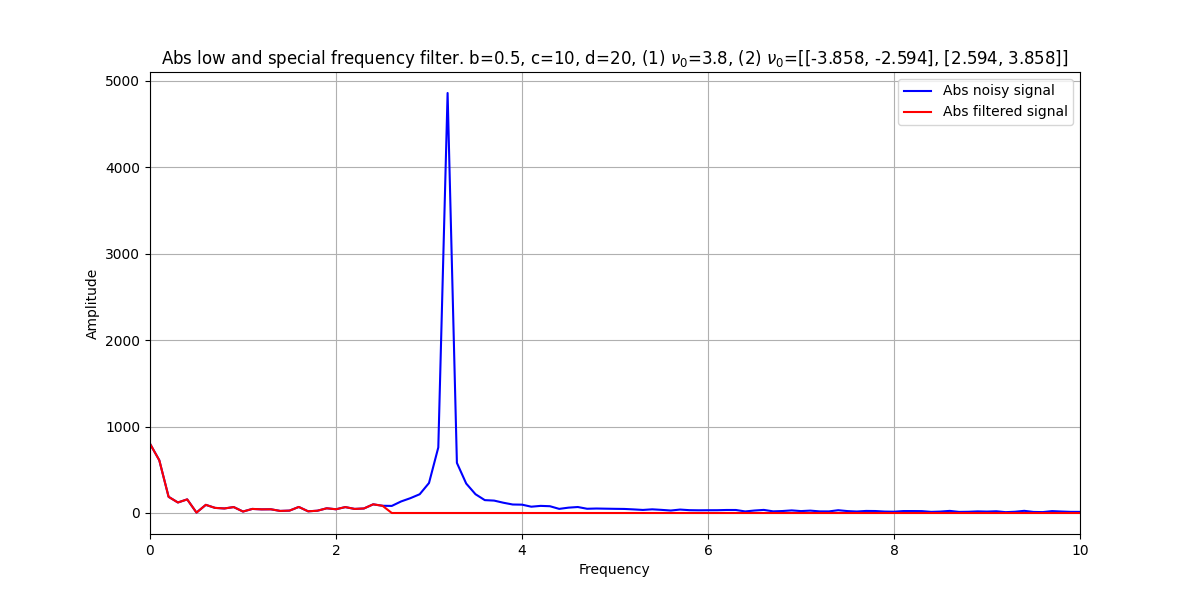
\includegraphics[scale=0.48]{3_abs_nospec_nohigh.png}
        \captionsetup{skip=0pt}
        \caption{График модуля Фурье-образа исходного и фильтрованного сигналов (3.2)}
        \label{fig:fig7823}
    \end{figure}
    \begin{figure}[H]
        \centering
        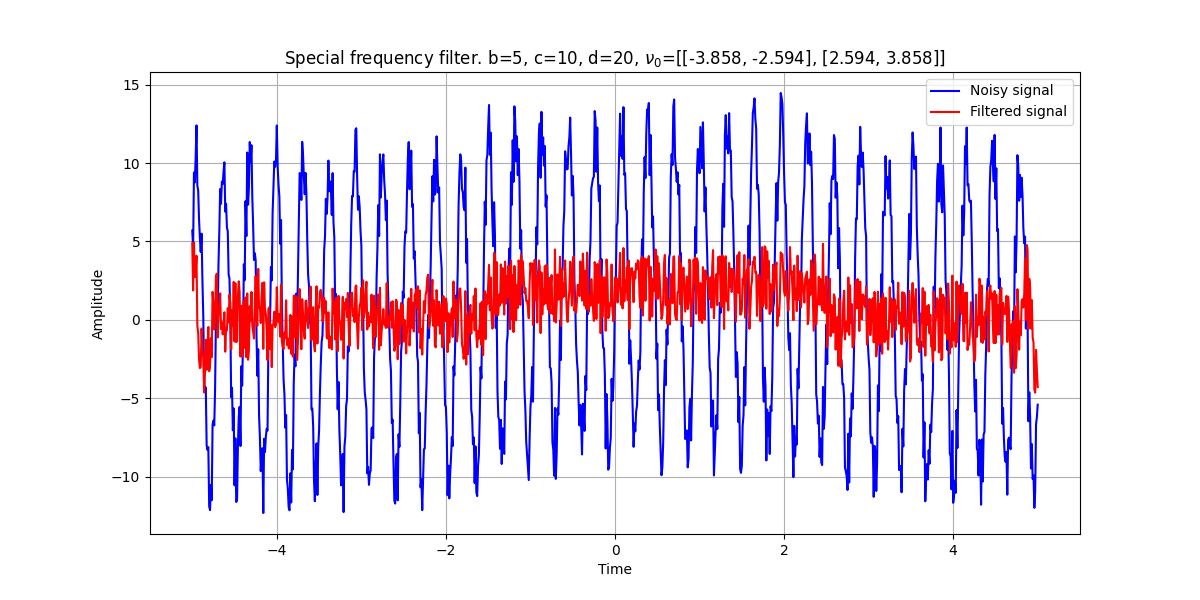
\includegraphics[scale=0.48]{4_nospec.png}
        \captionsetup{skip=0pt}
        \caption{График исходного и фильтрованного сигналов (4.1)}
        \label{fig:fig71234}
    \end{figure}
    \begin{figure}[H]
        \centering
        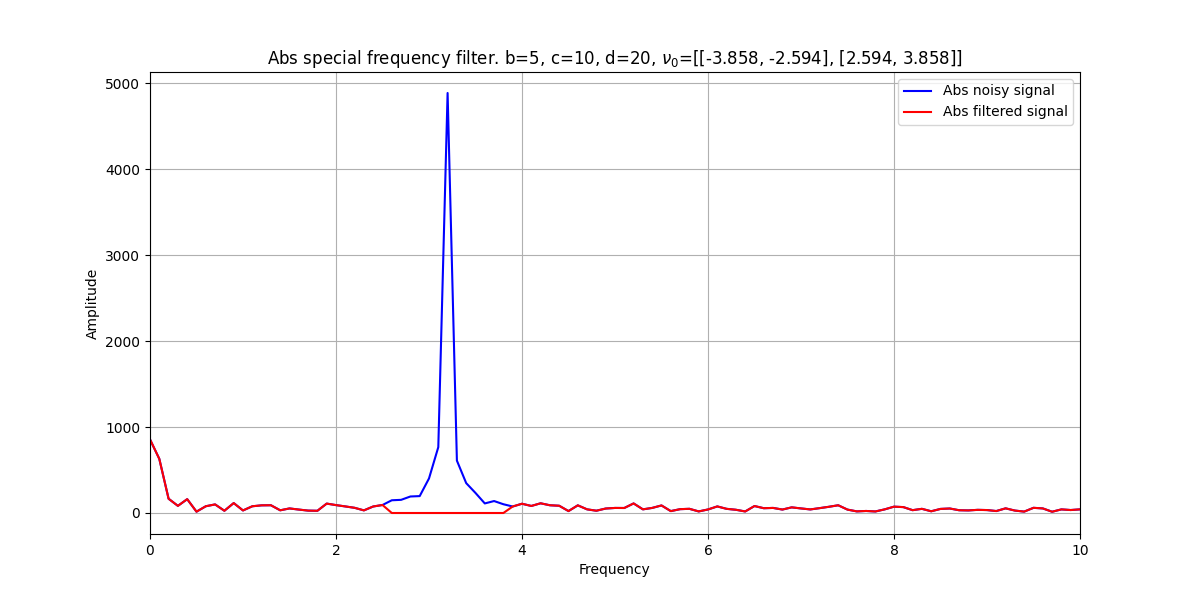
\includegraphics[scale=0.48]{4_abs_nospec.png}
        \captionsetup{skip=0pt}
        \caption{График модуля Фурье-образа исходного и фильтрованного сигналов (4.1)}
        \label{fig:fig72234}
    \end{figure}
    \begin{figure}[H]
        \centering
        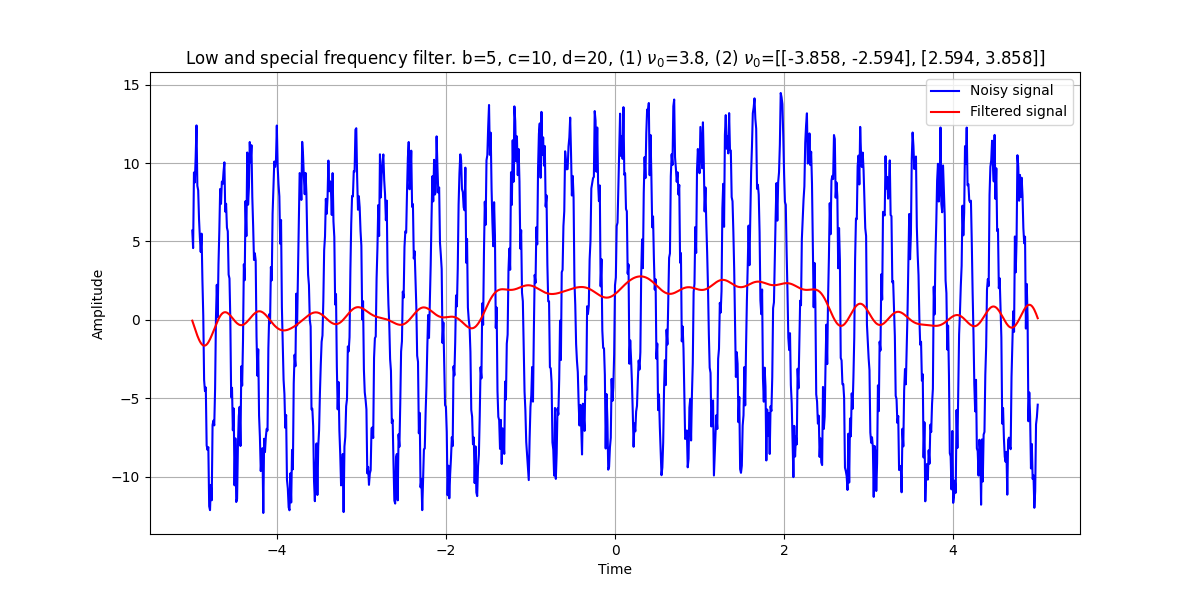
\includegraphics[scale=0.48]{4_nospec_nohigh.png}
        \captionsetup{skip=0pt}
        \caption{График исходного и фильтрованного сигналов (4.2)}
        \label{fig:fig77234}
    \end{figure}
    \begin{figure}[H]
        \centering
        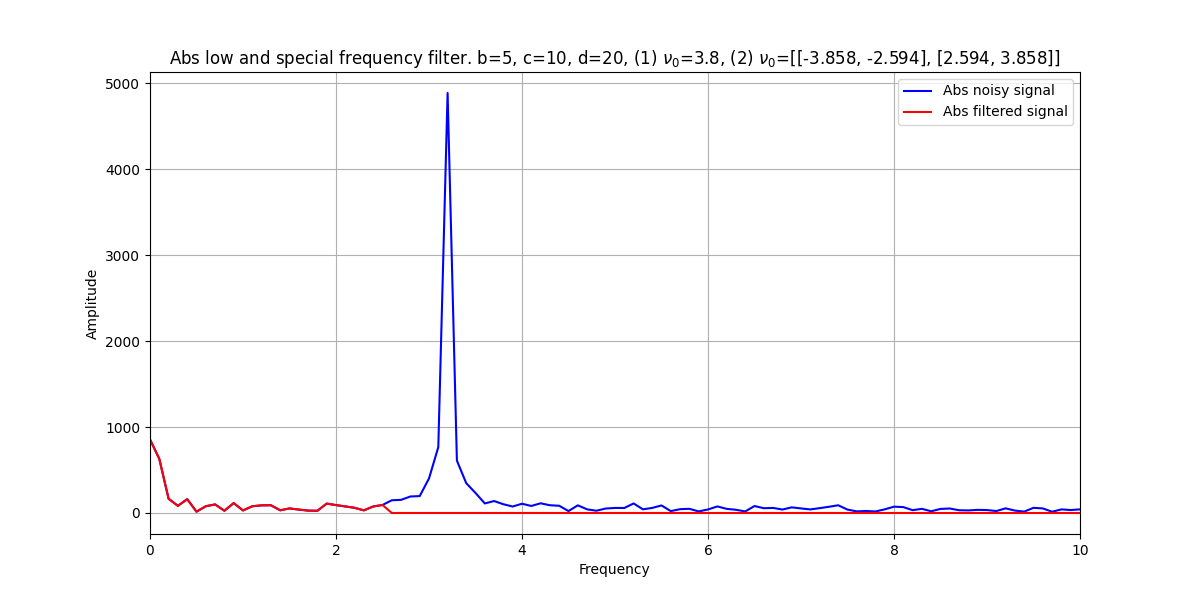
\includegraphics[scale=0.48]{4_abs_nospec_nohigh.png}
        \captionsetup{skip=0pt}
        \caption{График модуля Фурье-образа исходного и фильтрованного сигналов (4.2)}
        \label{fig:fig78234}
    \end{figure}
    \begin{figure}[H]
        \centering
        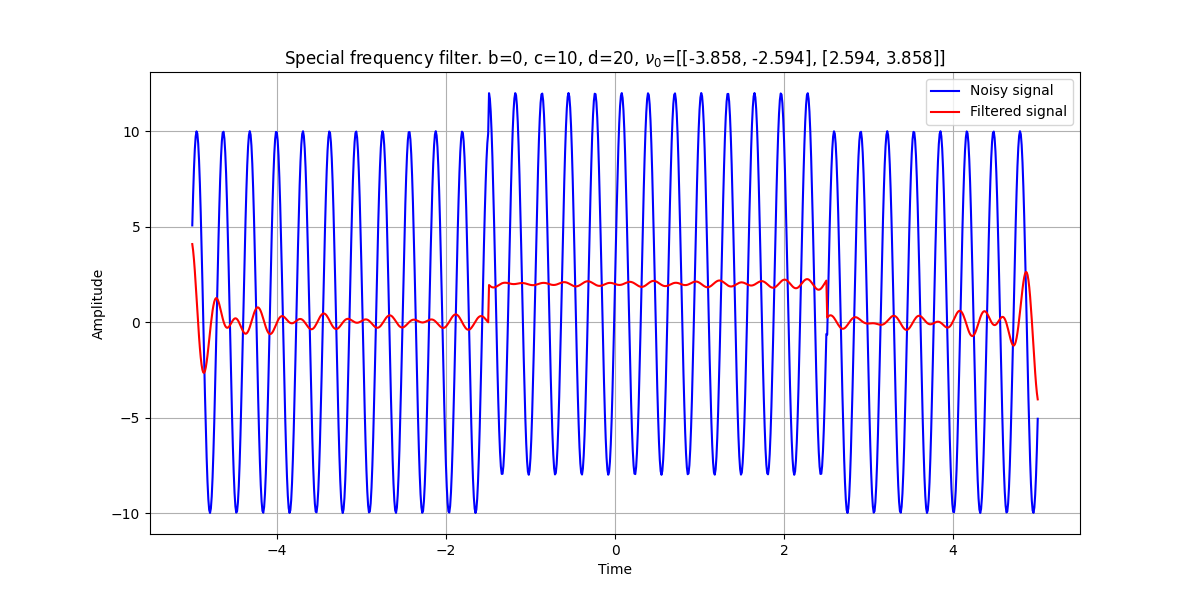
\includegraphics[scale=0.48]{5_nospec.png}
        \captionsetup{skip=0pt}
        \caption{График исходного и фильтрованного сигналов (5.1)}
        \label{fig:fig712345}
    \end{figure}
    \begin{figure}[H]
        \centering
        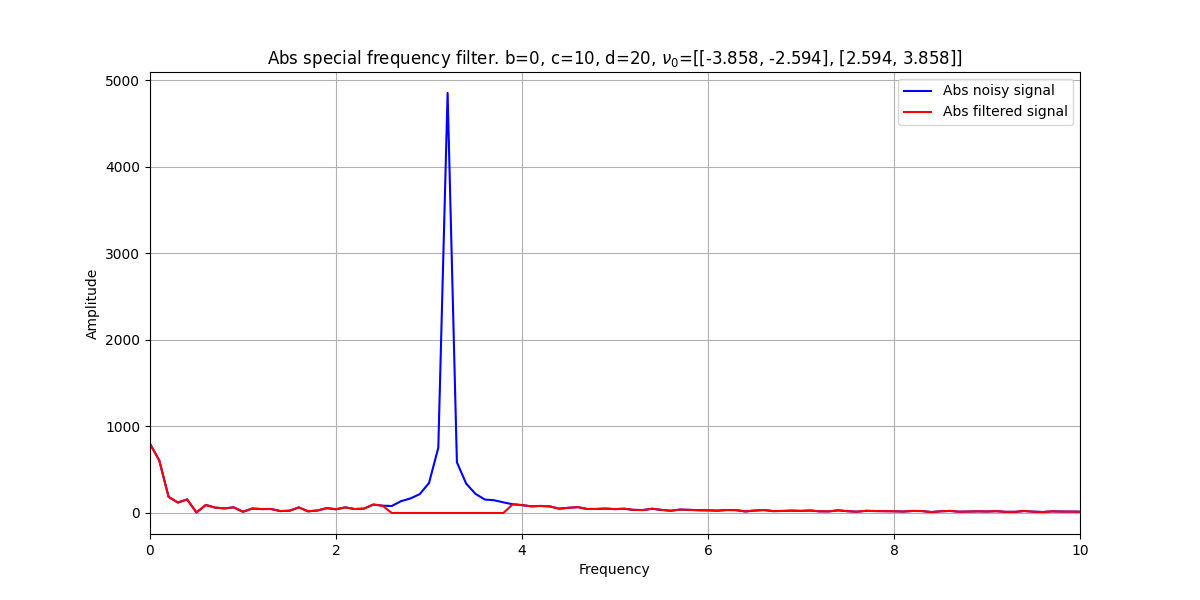
\includegraphics[scale=0.48]{5_abs_nospec.png}
        \captionsetup{skip=0pt}
        \caption{График модуля Фурье-образа исходного и фильтрованного сигналов (5.1)}
        \label{fig:fig722345}
    \end{figure}
    \begin{figure}[H]
        \centering
        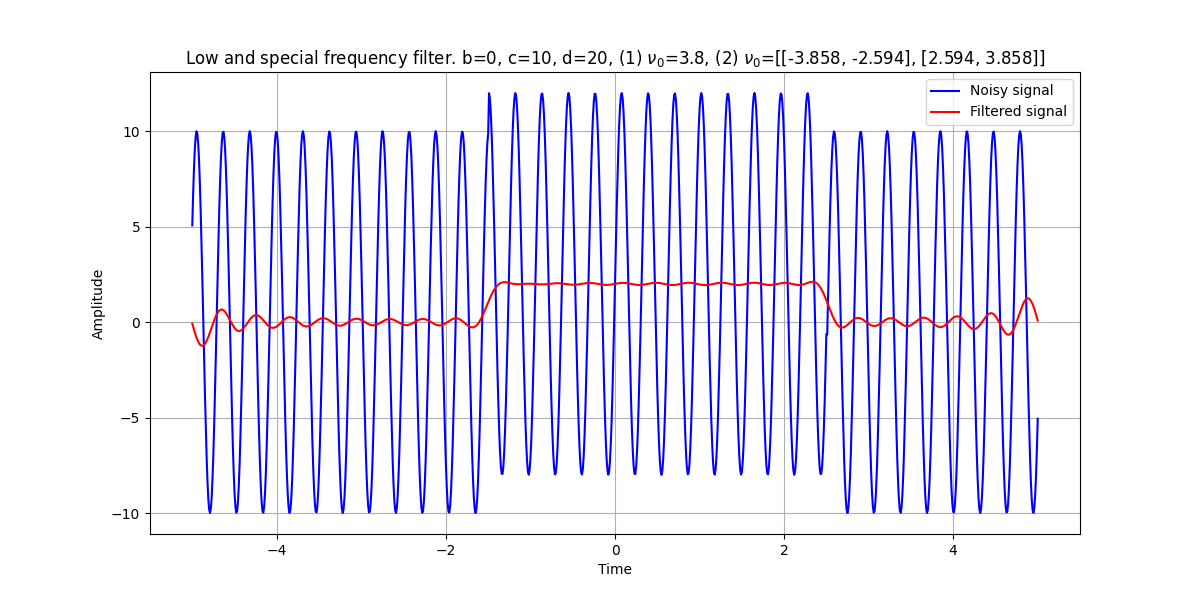
\includegraphics[scale=0.48]{5_nospec_nohigh.png}
        \captionsetup{skip=0pt}
        \caption{График исходного и фильтрованного сигналов (5.2)}
        \label{fig:fig772345}
    \end{figure}
    \begin{figure}[H]
        \centering
        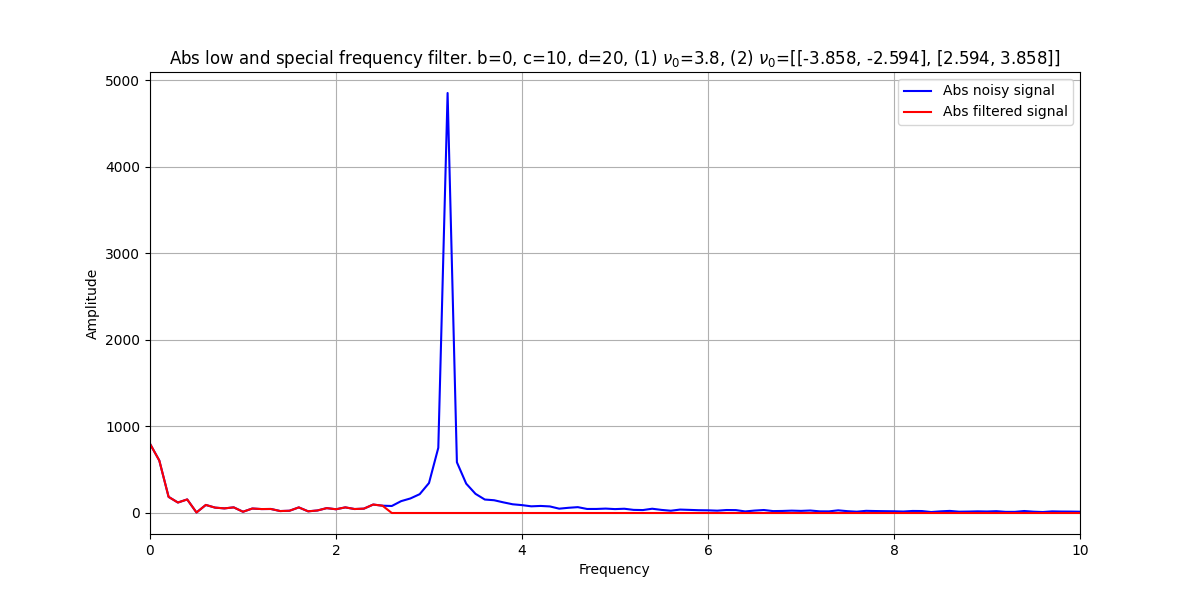
\includegraphics[scale=0.48]{5_abs_nospec_nohigh.png}
        \captionsetup{skip=0pt}
        \caption{График модуля Фурье-образа исходного и фильтрованного сигналов (5.2)}
        \label{fig:fig782345}
    \end{figure}


    Исходя из графиков можно сделать вывод, что параметр $c$ отвечает за синусоидальный шум. При увеличении параметра $c$
    сигнал во временной области растягивается по оси $Oy$, то есть возрастает амплитуда волн (сравн. рис. \ref{fig:fig712}, \ref{fig:fig7123}).
    На графиках Фурье-образов амплитуды также становятся больше (сравн. рис. \ref{fig:fig722}, \ref{fig:fig7223}). Затрудняет фильтрацию
    при больших значениях.


    Параметр $d$ характеризует растяжение сигнала во временной области по оси $Ox$. При увеличении его значения частота волн повышается.
    На графиках Фурье-образов увеличение значения параметра $d$ удаляет от нижних частот высокий пик, отвечающий за
    гармонический шум (сравн. рис. \ref{fig:fig72}, \ref{fig:fig722}), что упрощает фильтрацию сигнала, так как, например, на рис. \ref{fig:fig72}
    синусоидальный шум находится в том же месте, где наибольшее количество информации о сигнале -- его удаление приведет к потере некоторой информации об исходном сигнале,
    восстановленный будет выглядеть хуже, чем при б\'{о}льших значениях параметра $d$.


    Чем меньше $b$, тем меньше белого шума и проще восстанавливать сигнал.
    При $b=0$ сигнал $u$ описывается формулой синусоиды $$u=g+c\cdot\sin{(d\cdot t+0)},$$
    что можно увидеть на рис. \ref{fig:fig712345}.


    Как виды помехи параметры можно назвать так: $b$ -- белый шум, $c \text{ и } d$ гармонический шум.

    
    Наилучшей фильтрации мне удалось достичь при совмещении фильтра специфических и нижних частот.
   

    \subsection{Убираем низкие частоты. Фильтр верхних частот.}
    Рассмотрим графики, где в некоторой окресности точки $\nu=0$ обнулим все значения частот Фурье-образа.
    Такое поведение соответствует фильтру \textit{верхних} частот, так как он пропускает все частоты выше частоты среза.
    Окресность будет настраиваться выбором диапазона частот $[-\nu_0,\nu_0]$.


    Далее будут приведены рисунки полученных графиков. На каждом графике подписаны выбранные значения $b,\,c,\,d,\,\nu_0$. 
    Синим цветом обозначается оригинальный сигнал, красным фильтрованный.


    \begin{figure}[H]
        \centering
        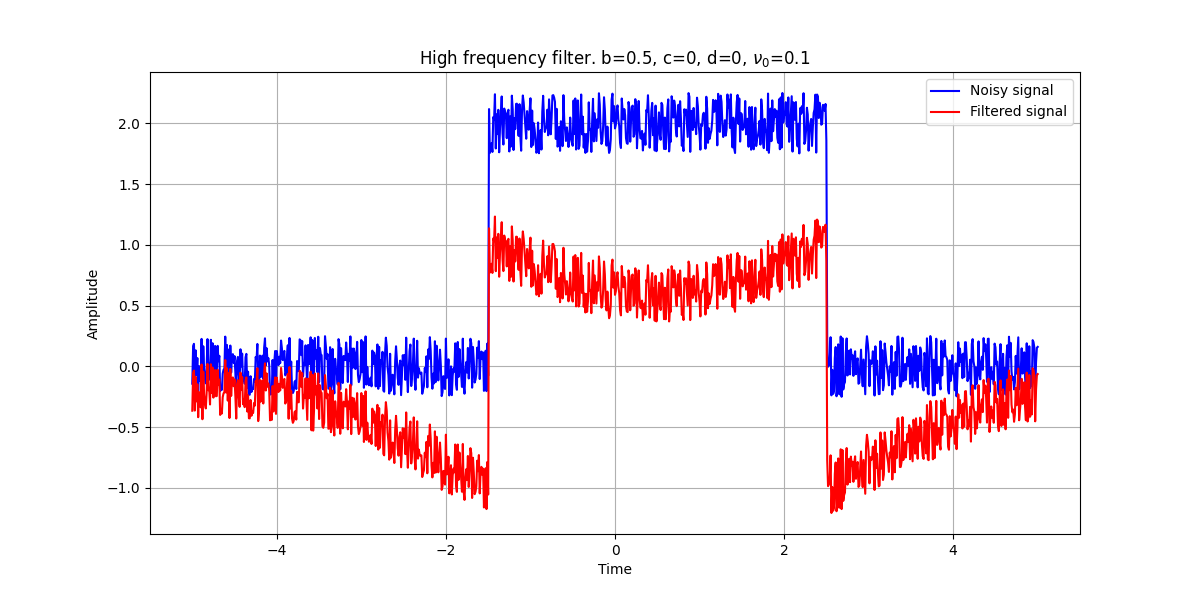
\includegraphics[scale=0.48]{1_nolow.png}
        \captionsetup{skip=0pt}
        \caption{График исходного и фильтрованного сигналов (1)}
        \label{fig:fig27}
    \end{figure}
    \begin{figure}[H]
        \centering
        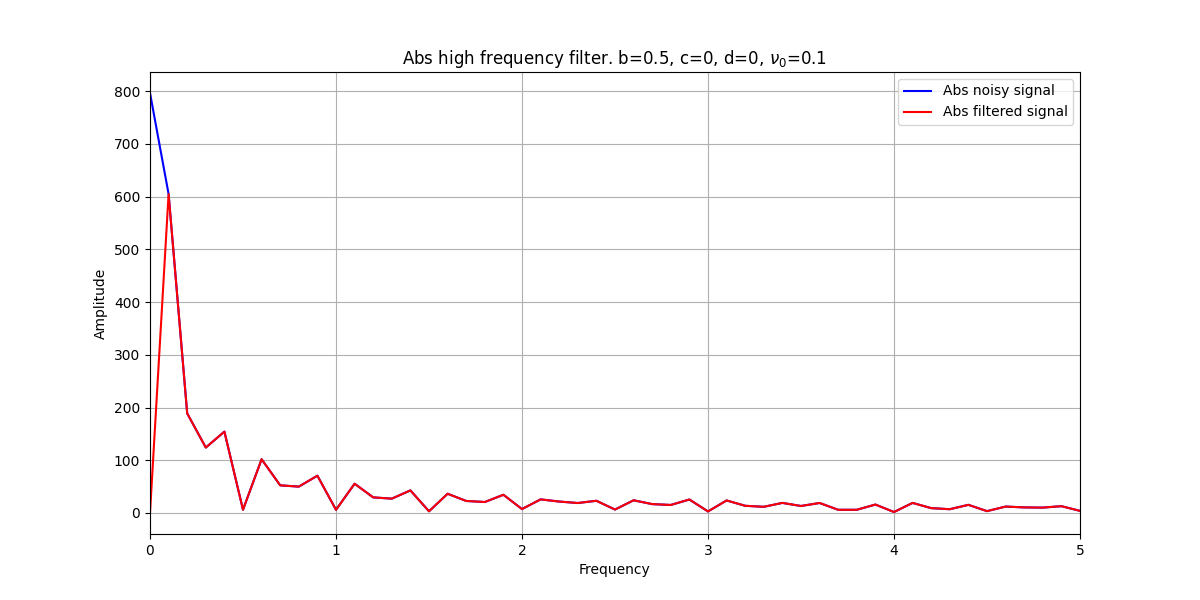
\includegraphics[scale=0.48]{1_abs_nolow.png}
        \captionsetup{skip=0pt}
        \caption{График модуля Фурье-образа исходного и фильтрованного сигналов (1)}
        \label{fig:fig28}
    \end{figure}
    \begin{figure}[H]
        \centering
        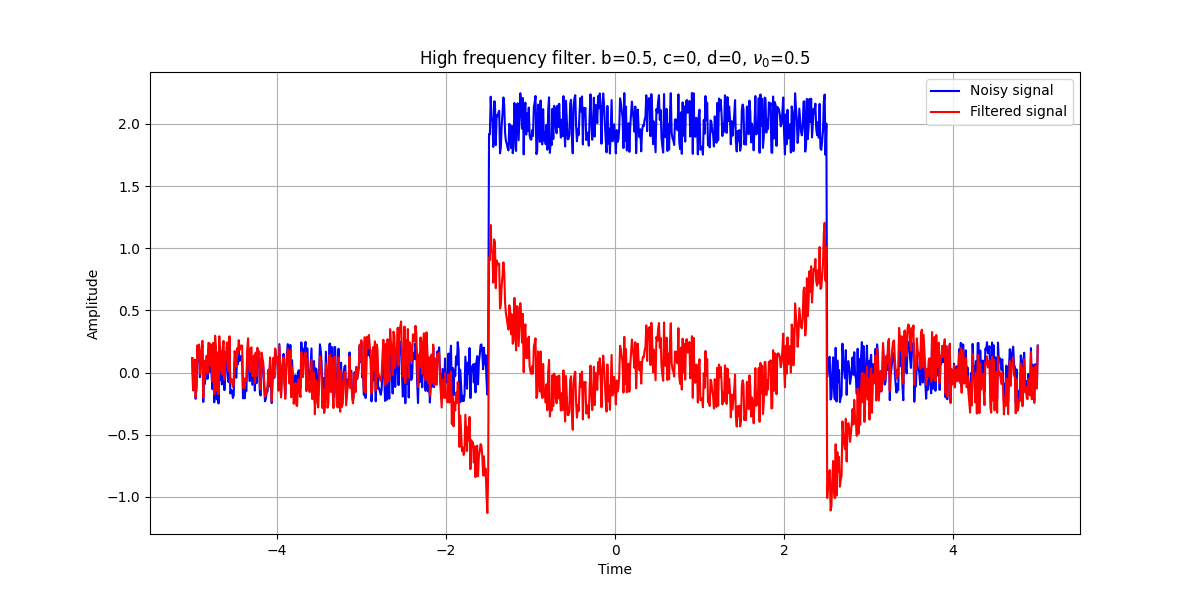
\includegraphics[scale=0.48]{2_nolow.png}
        \captionsetup{skip=0pt}
        \caption{График исходного и фильтрованного сигналов (2)}
        \label{fig:fig29}
    \end{figure}
    \begin{figure}[H]
        \centering
        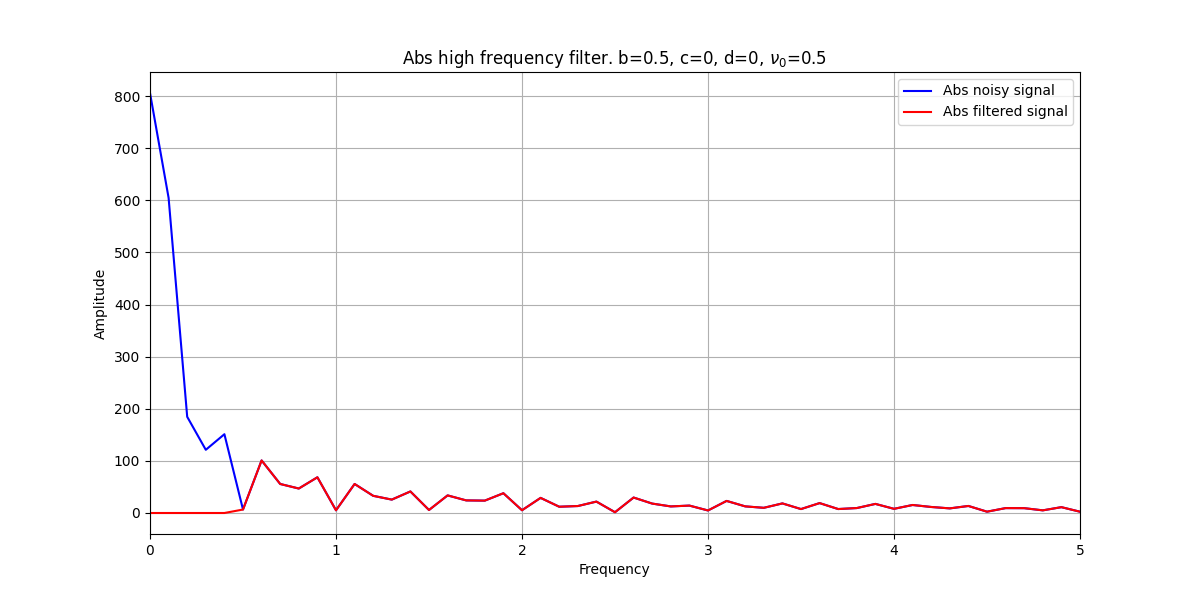
\includegraphics[scale=0.48]{2_abs_nolow.png}
        \captionsetup{skip=0pt}
        \caption{График модуля Фурье-образа исходного и фильтрованного сигналов (2)}
        \label{fig:fig30}
    \end{figure}
    \begin{figure}[H]
        \centering
        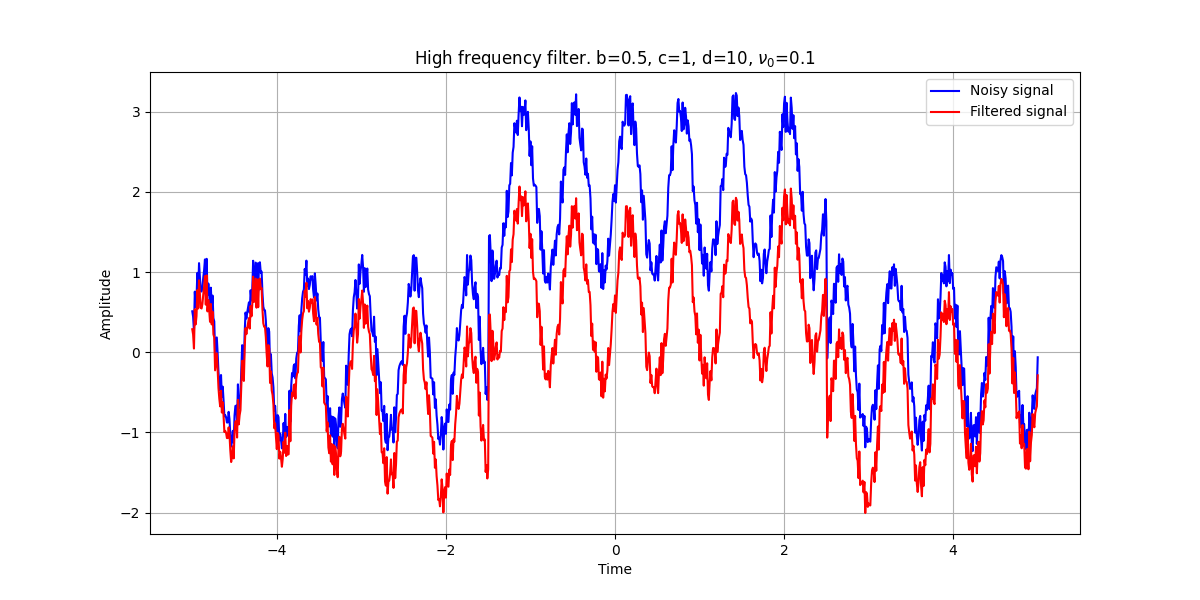
\includegraphics[scale=0.48]{3_nolow.png}
        \captionsetup{skip=0pt}
        \caption{График исходного и фильтрованного сигналов (3)}
        \label{fig:fig31}
    \end{figure}
    \begin{figure}[H]
        \centering
        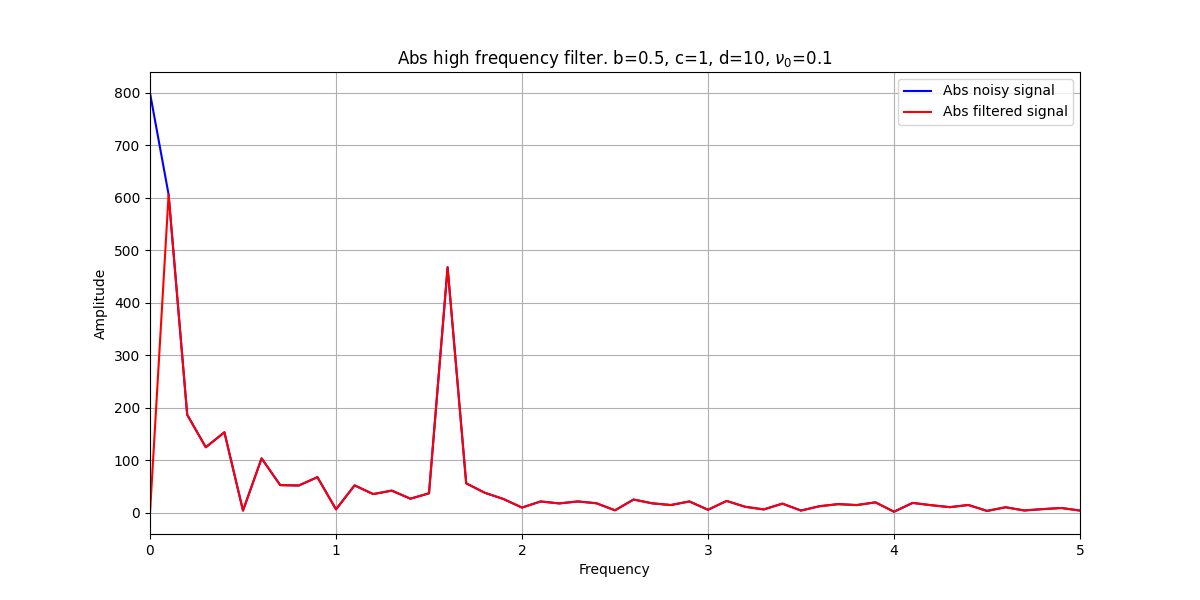
\includegraphics[scale=0.48]{3_abs_nolow.png}
        \captionsetup{skip=0pt}
        \caption{График модуля Фурье-образа исходного и фильтрованного сигналов (3)}
        \label{fig:fig32}
    \end{figure}
    \begin{figure}[H]
        \centering
        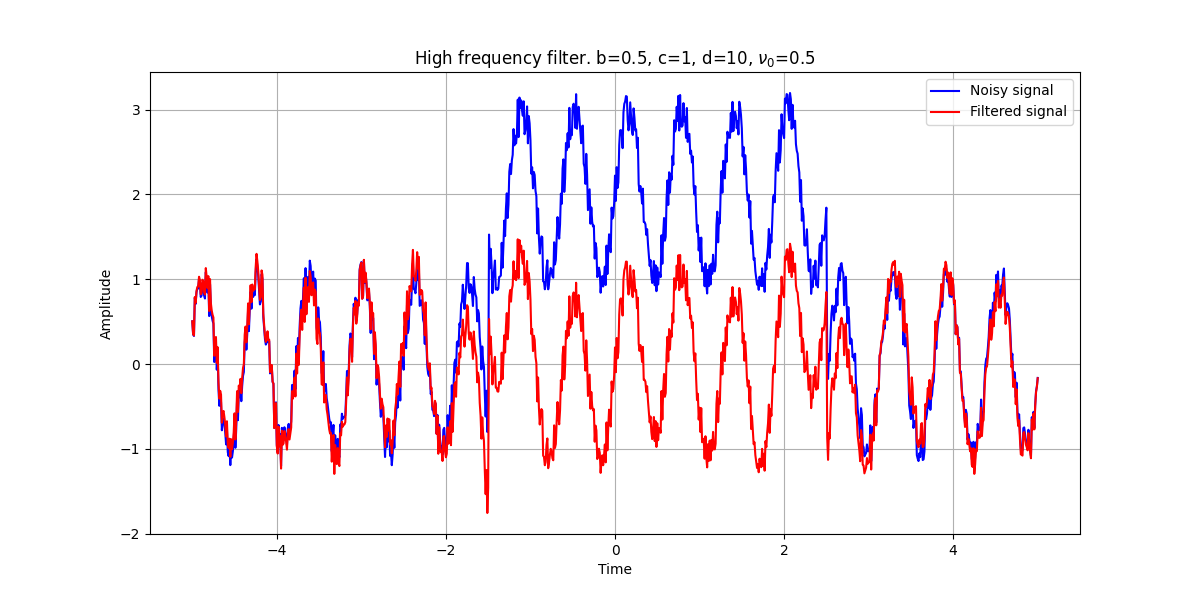
\includegraphics[scale=0.48]{4_nolow.png}
        \captionsetup{skip=0pt}
        \caption{График исходного и фильтрованного сигналов (4)}
        \label{fig:fig33}
    \end{figure}
    \begin{figure}[H]
        \centering
        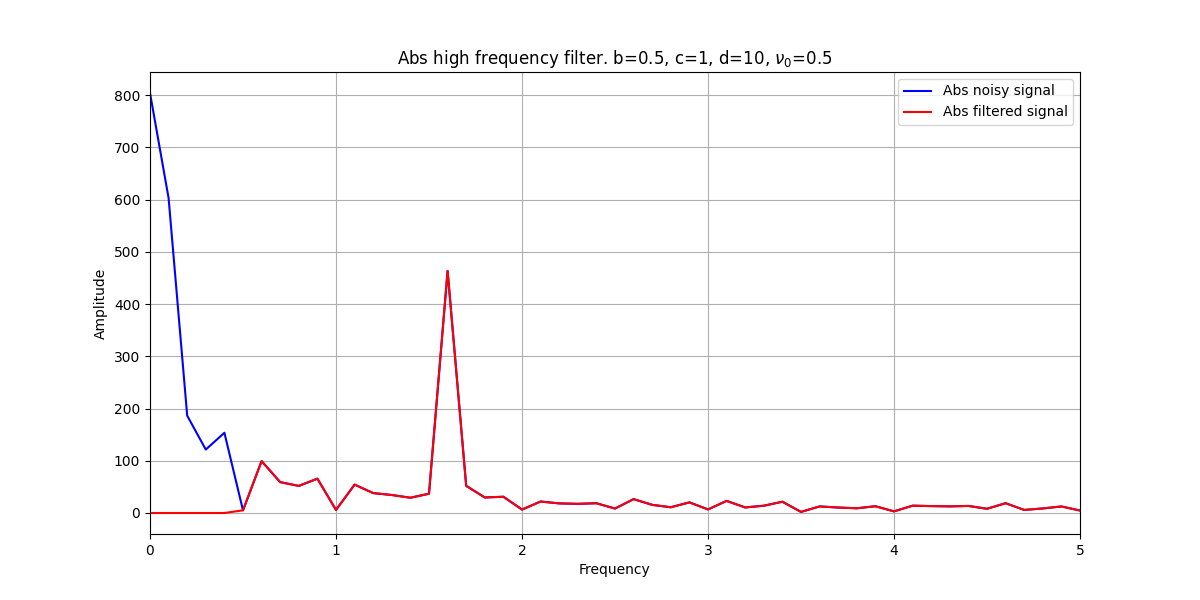
\includegraphics[scale=0.48]{4_abs_nolow.png}
        \captionsetup{skip=0pt}
        \caption{График модуля Фурье-образа исходного и фильтрованного сигналов (4)}
        \label{fig:fig34}
    \end{figure}
    
    
    По полученным графикам можно сделать вывод, что фильтр верхних частот в данном случае отрезает значимую часть сигнала,
    содержащуюся в нижних частотах, и оставляет только белый и/или гармонический шум, находящийся преимущественно на высоких частотах.
    Например, на рис. \ref{fig:fig33} видно, что фильтрованный сигнал почти не имеет подъема на том промежутке, где он должен быть, то есть
    почти вся информация о том, что сигнал имел подъем, была вырезана (см. рис. \ref{fig:fig34}).
    Следовательно, для заданного сигнала $u$ такой фильтр не
    подходит для восстановления исходного сигнала.


    \section{Задание 2. Фильтрация звука.}
    Построим графики исходного сигнала аудиозаписи и его Фурье-образа.
    На записи присутствует громкий гул, следовательно необходимо вырезать частоты из аудиозаписи, имеющие наибольшую амплитуду.
    \begin{figure}[H]
        \centering
        \begin{subfigure}{0.45\textwidth}
            \centering
            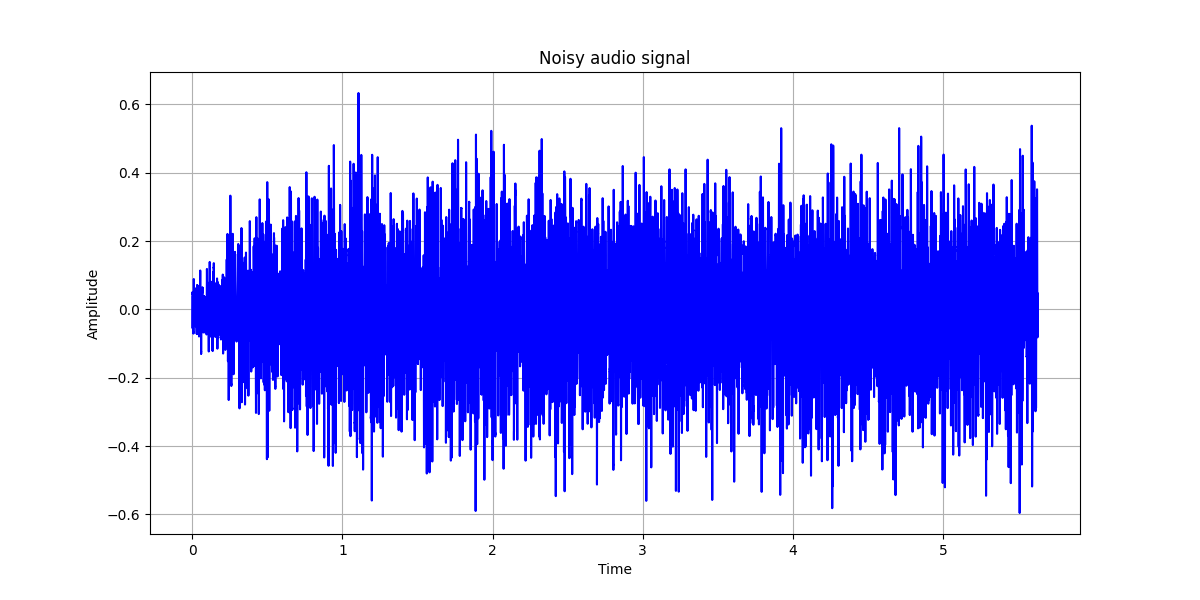
\includegraphics[width=\linewidth]{audio.png}
            \caption{Временная область}
            \label{fig:fig111}
        \end{subfigure}
        \hspace{5mm}
        \begin{subfigure}{0.45\textwidth}
            \centering
            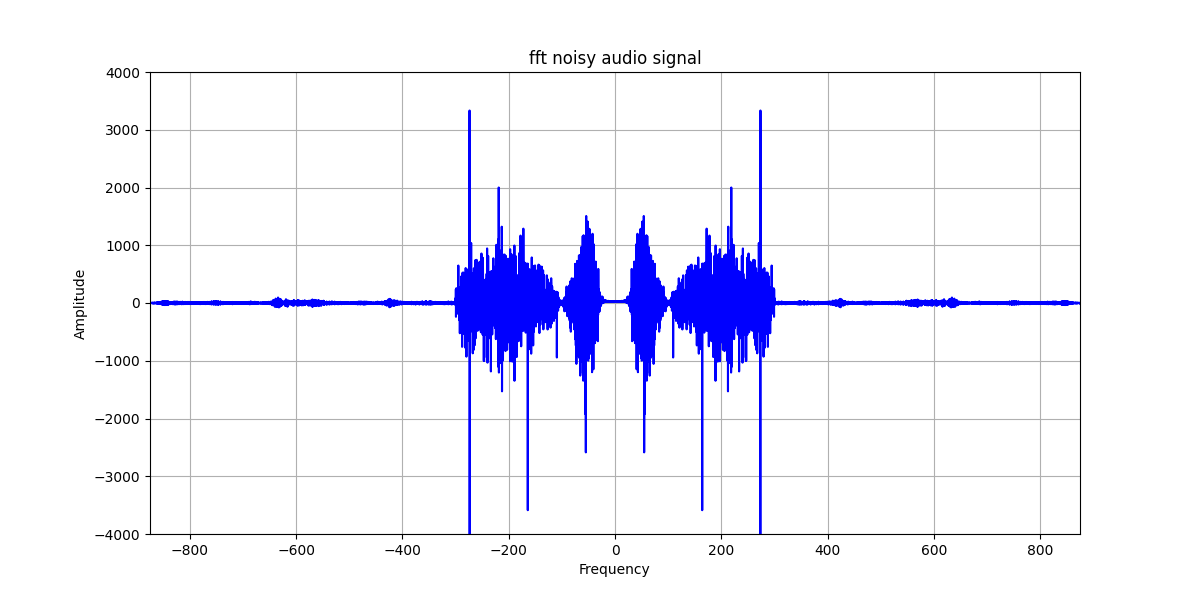
\includegraphics[width=\linewidth]{U_audio.png}
            \caption{Частотная область}
            \label{fig:fig112}
        \end{subfigure}
        \caption{Графики исходного сигнала и его Фурье-образа}
        \label{fig:timefreq0}
    \end{figure}
    
    
    Определим по второму графику, какие частоты могут создавать шумы.
    Самые большие амплитуды находятся в диапазоне частот $[-300,300]$ Гц. Чтобы их вырезать, потребуется фильтр верхних частот, который
    мы рассматривали в задании 1. Применим фильтр и посмотрим результирующие графики.
    \begin{figure}[H]
        \centering
        \begin{subfigure}{0.45\textwidth}
            \centering
            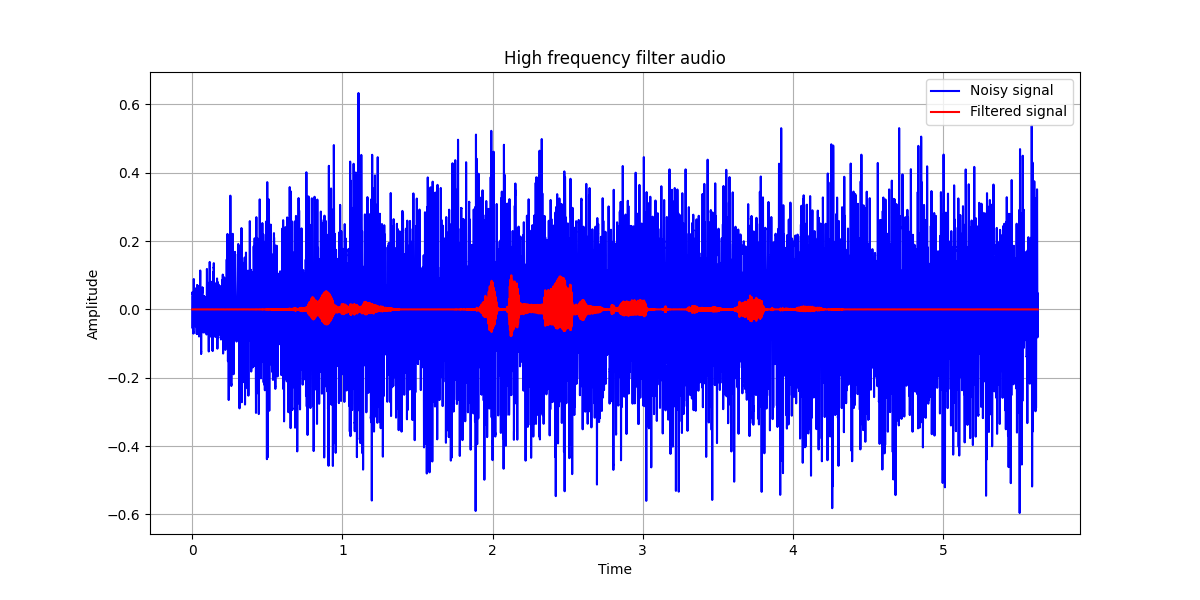
\includegraphics[width=\linewidth]{faudio.png}
            \caption{Временная область}
            \label{fig:fig113}
        \end{subfigure}
        \hspace{5mm}
        \begin{subfigure}{0.45\textwidth}
            \centering
            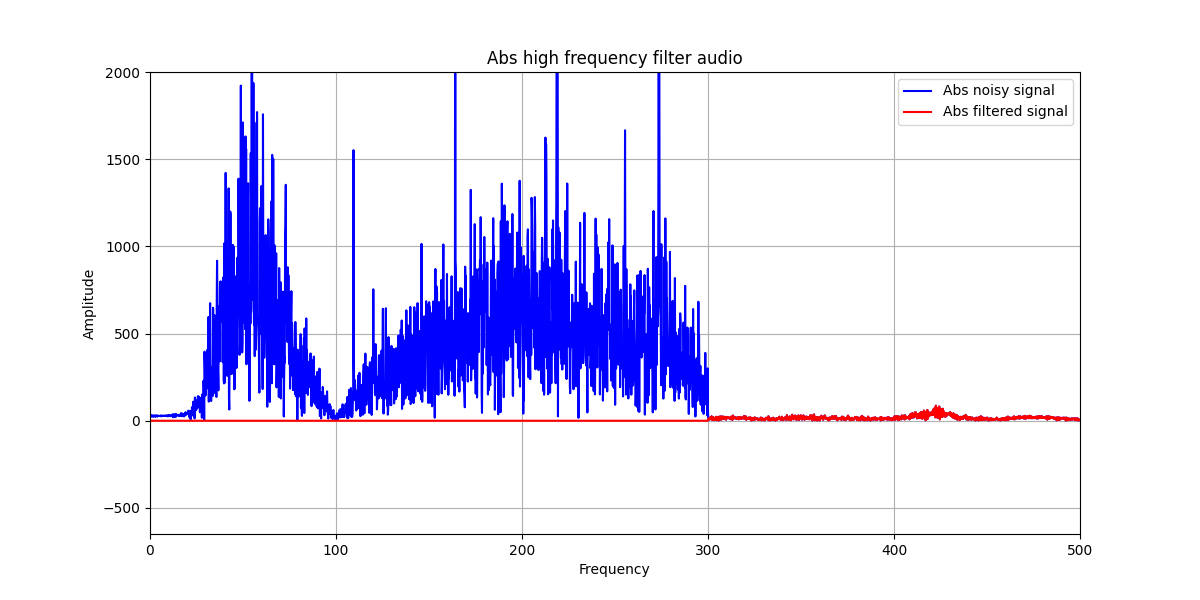
\includegraphics[width=\linewidth]{abs_audio.png}
            \caption{Частотная область}
            \label{fig:fig114}
        \end{subfigure}
        \caption{Графики исходного и фильтрованного сигналов и модулей их Фурье-образов}
        \label{fig:timefreq}
    \end{figure}

    
    Видим как из сигнала во временной области пропал белый шум -- оставшиеся амплитуды являются голосом, который 
    мы хотели хорошо расслышать.
    На графике модулей Фурье-образов наблюдаем, что мы вырезали
    низкие частоты с наибольшей амплитудой, которые соответствовали громкому гулу. Запись filtered\_{MUHA}.wav можно послушать,
    на этом \href{https://drive.google.com/drive/folders/1AuXIiKRWvXFOtJqV3uqPzC494zZ7vCrd?usp=sharing}{гугл-диске}.
    На записи голос слышно хорошо, однако остался некоторый звуковой эффект фейзер.

    
    \section{Листинги программных реализаций}
    Все программы написаны на языке python с подключенными библиотеками numpy и matplotlib.

    
    Два файла, которые необходимы для задания массива времени и частот, вычисления массива функций $g$, задания
    сигнала $u$, а также подсчета Фурье-образа сигнала $u$. Достаточно передать в функции необходимые параметры и
    далее их результат можно использовать для выполнения фильтрации и построения графиков.
    \begin{lstlisting}[label=l1, caption={Файл help.py. Вспомогательные функции}]
    def get_t(T, dt):
        return np.arange(-T/2, T/2 + dt, dt)   
        
    def get_v(V, dv):
        return np.arange(-V/2, V/2 + dv, dv)
          
    def get_U(u):
        return np.fft.fftshift(np.fft.fft(u))
        
    def g_f(t, t_1, t_2, a):
        if (t_1 <= t <= t_2):
            return a
        return 0
        
    def u_f(g_fs: list, time: list, b, c, d):
        return np.array(g_fs) + \
               b*(np.random.rand(len(time))-0.5) + \
               c*np.sin(d*time)
        
    def get_g_fs(time: list, t_1, t_2, a):
        gs = []
        for t in range(len(time)):
            gs.append(g_f(time[t], t_1, t_2, a))
        
        return gs   
    \end{lstlisting}
    \begin{lstlisting}[label=l2, caption={Файл static.py. Вспомогательные переменные}]
    import help as hp

    a = 2
    t_1, t_2 = -1.5, 2.5

    T, dt = 10, 0.01
    V, dv = 1 / dt, 1 / T

    time = hp.get_t(T, dt)
    freq = hp.get_v(V, dv)
    g_fs = hp.get_g_fs(time, t_1, t_2, a)
    \end{lstlisting}


    Программа для построения сравнительных графиков исходного и фильтрованного сигналов и
    модулей их Фурье-образов.
    \begin{lstlisting}[label=l3, caption={Файл builder.py. Реализация построения графиков}]
    import matplotlib.pyplot as plt
    import numpy as np

    from help import get_U

    def build_u_to_U(freq: list,
                    u: list,
                    clr='b',
                    xl1=None,
                    xl2=None,
                    yl1=None,
                    yl2=None,
                    xlab='Frequency',
                    ylab='Amplitude',
                    label=None,
                    title=None,
                    fz1=6.4,
                    fz2=4.8,
                    legend: bool = True,
                    grid: bool = True):
        U = get_U(u)
        build_u_or_U(freq, U, clr, xl1, xl2,
                    yl1, yl2, xlab, ylab, label,
                    title, fz1, fz2, legend, grid)

    def build_u_or_U(torv: list,
                    uorU: list,
                    clr='b',
                    xl1=None,
                    xl2=None,
                    yl1=None,
                    yl2=None,
                    xlab=None,
                    ylab='Amplitude',
                    label=None,
                    title=None,
                    fz1=6.4,
                    fz2=4.8,
                    legend: bool = True,
                    grid: bool = True):
        plt.plot(torv, uorU, color=clr, label=label)
        plt.xlabel(xlab)
        plt.ylabel(ylab)
        plt.xlim(xl1, xl2)
        plt.ylim(yl1, yl2)
        plt.title(title)
        if legend:
            plt.legend()
        plt.grid(grid)
        plt.gcf().set_size_inches(fz1, fz2)
        plt.show()

    def build_u__flt_u(time: list,
                    u: list,
                    flt_u: list,
                    clr1='b',
                    clr2='r',
                    lab1='Noisy signal',
                    lab2='Filtered signal',
                    xlab='Time',
                    ylab='Amplitude',
                    title=None,
                    fz1=6.4,
                    fz2=4.8,
                    legend: bool = True,
                    grid: bool = True,
                    xl1=None,
                    xl2=None,
                    yl1=None,
                    yl2=None):
        plt.plot(time, u, color=clr1, label=lab1)
        plt.plot(time, flt_u, color=clr2, label=lab2)
        plt.xlabel(xlab)
        plt.ylabel(ylab)
        plt.xlim(xl1, xl2)
        plt.ylim(yl1, yl2)
        plt.title(title)
        if legend:
            plt.legend()
        plt.grid(grid)
        plt.gcf().set_size_inches(fz1, fz2)
        plt.show()

    def build_abs_u_to_U__flt_U(freq: list,
                                u: list,
                                flt_U: list,
                                clr1='b',
                                clr2='r',
                                lab1='Abs noisy signal',
                                lab2='Abs filtered signal',
                                xlab='Frequency',
                                ylab='Amplitude',
                                xl1=None,
                                xl2=None,
                                yl1=None,
                                yl2=None,
                                title=None,
                                fz1=6.4,
                                fz2=4.8,
                                legend: bool = True,
                                grid: bool = True):
        U = get_U(u)
        build_abs_U__flt_U(freq, U, flt_U, clr1,
                           clr2, lab1, lab2, xlab,
                           ylab, xl1, xl2, yl1, yl2,
                           title, fz1, fz2, legend, grid)

    def build_abs_U__flt_U(freq: list,
                        U: list,
                        flt_U: list,
                        clr1='b',
                        clr2='r',
                        lab1='Abs noisy signal',
                        lab2='Abs filtered signal',
                        xlab='Frequency',
                        ylab='Amplitude',
                        xl1=None,
                        xl2=None,
                        yl1=None,
                        yl2=None,
                        title=None,
                        fz1=6.4,
                        fz2=4.8,
                        legend: bool = True,
                        grid: bool = True):
        plt.plot(freq, np.abs(U), color=clr1, label=lab1)
        plt.plot(freq, np.abs(flt_U), color=clr2, label=lab2)
        plt.xlabel(xlab)
        plt.ylabel(ylab)
        plt.xlim(xl1, xl2)
        plt.ylim(yl1, yl2)
        plt.title(title)
        if legend:
            plt.legend()
        plt.grid(grid)
        plt.gcf().set_size_inches(fz1, fz2)
        plt.show()
    \end{lstlisting}


    Программа, реализующая методы фильтрации верхних, нижних и специфических частот.
    Здесь реализован алгоритм, описанный в первом задании -- вычисляется Фурье-образ,
    фильтруется и преобразуется обратно из частотного пространства во временное.
    \begin{lstlisting}[label=l4, caption={Файл filters.py. Реализация фильтров}]
    def filter_U(u: list, freq: list, v_0, filter):
        flt_U = get_U(u)
        for i in range(len(freq)):
            freq_i = freq[i]
            if filter(freq_i, v_0):
                flt_U[i] = 0
    
        return flt_U
    
    def low_filter(freq, v_0):
        if -v_0 <= freq <= v_0:
            return False
        return True
    
    def high_filter(freq, v_0):
        return not low_filter(freq, v_0)
    
    def special_filter_in(freq, v_0: list):
        for i in range(len(v_0)):
            if v_0[i][0] <= freq <= v_0[i][1]:
                return False
        return True

    def special_filter_out(freq, v_0: list):
        return not special_filter_in(freq, v_0)
    
    def filter_low(freq: list, u: list, v_0):
        if isinstance(v_0, list) or \
                len(freq) <= 0 or \
                len(u) <= 0:
            return None
    
        flt_U = filter_U(u, freq, v_0, low_filter)
        flt_u = np.fft.ifft(np.fft.ifftshift(flt_U))
        return flt_u, flt_U
    
    def filter_high(freq: list, u: list, v_0):
        if isinstance(v_0, list) or \
                len(freq) <= 0 or \
                len(u) <= 0:
            return None
    
        flt_U = filter_U(u, freq, v_0, high_filter)
        flt_u = np.fft.ifft(np.fft.ifftshift(flt_U))
        return flt_u, flt_U
    
    def filter_special_in(freq: list, u: list, v_0: list):
        if not isinstance(v_0, list) or \
                len(v_0) <= 0 or \
                len(freq) <= 0 or \
                len(u) <= 0:
            return None
    
        flt_U = filter_U(u, freq, v_0, special_filter_in)
        flt_u = np.fft.ifft(np.fft.ifftshift(flt_U))
        return flt_u, flt_U

    def filter_special_out(freq: list, u: list, v_0: list):
        if not isinstance(v_0, list) or \
                len(v_0) <= 0 or \
                len(freq) <= 0 or \
                len(u) <= 0:
            return None
    
        flt_U = filter_U(u, freq, v_0, special_filter_out)
        flt_u = np.fft.ifft(np.fft.ifftshift(flt_U))
        return flt_u, flt_U
    \end{lstlisting}


    Далее представлены программы, в которых используются все предыдущие наработки. Типовой алгоритм -- задать
    параметры $b,\,c,\,d$ и некоторый $\nu_0$, далее воспользоваться функциями создания зашумленного сигнала,
    фильтрации нужных частот и построения необходимых графиков.
    Для работы с аудиозаписью подключены библиотеки librosa, scipy и playsound.
    \begin{lstlisting}[label=l5, caption={Файл nohigh.py. Фильтрация нижних частот}]
    import help as hp
    import static as st

    import filters as ft
    import builder as bd

    time = st.time
    freq = st.freq
    g_fs = st.g_fs

    b, c, d = 0.5, 0, 0.1
    v_0 = 2.5

    u = hp.u_f(g_fs, time, b, c, d)
    flt_u, flt_U = ft.filter_low(freq, u, v_0)

    bd.build_u__flt_u(
        time,
        u,
        flt_u,
        title=rf'Low frequency filter. b={b}, c={c}, d={d}, $\nu_0$={v_0}',
        fz1=12,
        fz2=6)
    bd.build_abs_u_to_U__flt_U(
        freq,
        u,
        flt_U,
        title=
        rf'Abs low frequency filter. b={b}, c={c}, d={d}, $\nu_0$={v_0}',
        xl1=-5,
        xl2=5,
        fz1=12,
        fz2=6)
    \end{lstlisting}


    \begin{lstlisting}[label=l6, caption={Файл nolow.py. Фильтрация верхних частот}]
    import help as hp
    import static as st

    import filters as ft
    import builder as bd

    time = st.time
    freq = st.freq
    g_fs = st.g_fs

    b, c, d = 5, 10, 0.5
    v_0 = 0.3

    u = hp.u_f(g_fs, time, b, c, d)
    flt_u, flt_U = ft.filter_high(freq, u, v_0)

    bd.build_u__flt_u(
        time,
        u,
        flt_u,
        title=rf'High frequency filter. b={b}, c={c}, d={d}, $\nu_0$={v_0}',
        fz1=12,
        fz2=6)
    bd.build_abs_u_to_U__flt_U(
        freq,
        u,
        flt_U,
        title=
        rf'Abs high frequency filter. b={b}, c={c}, d={d}, $\nu_0$={v_0}',
        fz1=12,
        fz2=6,
        xl1=-5,
        xl2=5)
    \end{lstlisting}


    \begin{lstlisting}[label=l7, caption={Файл nospec.py. Фильтрация специфических частот}]
    import help as hp
    import static as st

    import filters as ft
    import builder as bd

    time = st.time
    freq = st.freq
    g_fs = st.g_fs

    b, c, d = 1.5, -2, -3
    v0, v01 = [[-0.52, -0.3], [0.3, 0.52]], 10
    u = hp.u_f(g_fs, time, b, c, d)

    flt_u_so, flt_U_so = ft.filter_special_out(freq, u, v0)
    bd.build_u__flt_u(
        time,
        u,
        flt_u_so.real,
        title=
        rf'Special frequency filter. b={b}, c={c}, d={d}, $\nu_0$={v0}',
        fz1=12,
        fz2=6)
    bd.build_abs_u_to_U__flt_U(
        freq,
        u,
        flt_U_so,
        title=
        rf'Abs special frequency filter. b={b}, c={c}, d={d}, $\nu_0$={v0}',
        fz1=12,
        fz2=6,
        xl1=-10,
        xl2=10)

    flt_u_lso, flt_U_lso = ft.filter_low(freq, flt_u_so, v01)
    bd.build_u__flt_u(
        time,
        u,
        flt_u_lso.real,
        title=
        rf'Low and special frequency filter. b={b}, c={c}, d={d}, (1) $\nu_0$={v01}, (2) $\nu_0$={v0}',
        fz1=12,
        fz2=6)
    bd.build_abs_u_to_U__flt_U(
        freq,
        u,
        flt_U_lso,
        title=
        rf'Abs low and special frequency filter. b={b}, c={c}, d={d}, (1) $\nu_0$={v01}, (2) $\nu_0$={v0}',
        fz1=12,
        fz2=6,
        xl1=-10 - v01,
        xl2=10 + v01)
    \end{lstlisting}


    \begin{lstlisting}[label=l8, caption={Файл audio.py. Фильтрация шумов в аудиозаписи}]
    import numpy as np
    import librosa
    from scipy.io.wavfile import write
    from playsound import playsound

    import filters as ft
    import builder as bd

    title = 'High frequency filter audio'
    title2 = 'Abs high frequency filter audio'

    src = 'fm_lab3/sound/MUHA.wav'
    filename = 'fm_lab3/sound/filtered_MUHA.wav'
    audio, rate = librosa.load(src, sr=None)

    dt = 1 / rate
    T = len(audio) * dt

    time = np.linspace(0, T, len(audio), endpoint=False)
    freq = np.linspace(-rate / 2, rate / 2, len(audio), endpoint=False)

    flt_u, flt_U = ft.filter_high(freq, audio, 300)
    flt_u_float = flt_u.real.astype(np.float32)

    bd.build_u_or_U(time,
                    audio,
                    xlab='Time',
                    title='Noisy audio signal',
                    fz1=12,
                    fz2=6,
                    legend=False)
    bd.build_u_to_U(freq,
                    audio,
                    title='fft noisy audio signal',
                    legend=False,
                    fz1=12,
                    fz2=6,
                    xl1=0,
                    yl1=0,
                    yl2=20)

    bd.build_u__flt_u(time, audio, flt_u, title=title, fz1=12, fz2=6)
    bd.build_abs_u_to_U__flt_U(freq,
                            audio,
                            flt_U,
                            title=title2,
                            fz1=12,
                            fz2=6,
                            xl1=0,
                            yl1=0,
                            yl2=20)

    write(filename, rate, flt_u_float)
    playsound(filename)
    \end{lstlisting}
\end{document}